\documentclass[twoside]{book}

% Packages required by doxygen
\usepackage{calc}
\usepackage{doxygen}
\usepackage{graphicx}
\usepackage[utf8]{inputenc}
\usepackage{makeidx}
\usepackage{multicol}
\usepackage{multirow}
\usepackage{textcomp}
\usepackage[table]{xcolor}

% Font selection
\usepackage[T1]{fontenc}
\usepackage{mathptmx}
\usepackage[scaled=.90]{helvet}
\usepackage{courier}
\usepackage{amssymb}
\usepackage{sectsty}
\renewcommand{\familydefault}{\sfdefault}
\allsectionsfont{%
  \fontseries{bc}\selectfont%
  \color{darkgray}%
}
\renewcommand{\DoxyLabelFont}{%
  \fontseries{bc}\selectfont%
  \color{darkgray}%
}

% Page & text layout
\usepackage{geometry}
\geometry{%
  a4paper,%
  top=2.5cm,%
  bottom=2.5cm,%
  left=2.5cm,%
  right=2.5cm%
}
\tolerance=750
\hfuzz=15pt
\hbadness=750
\setlength{\emergencystretch}{15pt}
\setlength{\parindent}{0cm}
\setlength{\parskip}{0.2cm}
\makeatletter
\renewcommand{\paragraph}{%
  \@startsection{paragraph}{4}{0ex}{-1.0ex}{1.0ex}{%
    \normalfont\normalsize\bfseries\SS@parafont%
  }%
}
\renewcommand{\subparagraph}{%
  \@startsection{subparagraph}{5}{0ex}{-1.0ex}{1.0ex}{%
    \normalfont\normalsize\bfseries\SS@subparafont%
  }%
}
\makeatother

% Headers & footers
\usepackage{fancyhdr}
\pagestyle{fancyplain}
\fancyhead[LE]{\fancyplain{}{\bfseries\thepage}}
\fancyhead[CE]{\fancyplain{}{}}
\fancyhead[RE]{\fancyplain{}{\bfseries\leftmark}}
\fancyhead[LO]{\fancyplain{}{\bfseries\rightmark}}
\fancyhead[CO]{\fancyplain{}{}}
\fancyhead[RO]{\fancyplain{}{\bfseries\thepage}}
\fancyfoot[LE]{\fancyplain{}{}}
\fancyfoot[CE]{\fancyplain{}{}}
\fancyfoot[RE]{\fancyplain{}{\bfseries\scriptsize Generated on Mon Dec 7 2015 10\-:14\-:06 for R\-A\-P\-P Platform Tests -\/ Speech Detection Sphinx4 by Doxygen }}
\fancyfoot[LO]{\fancyplain{}{\bfseries\scriptsize Generated on Mon Dec 7 2015 10\-:14\-:06 for R\-A\-P\-P Platform Tests -\/ Speech Detection Sphinx4 by Doxygen }}
\fancyfoot[CO]{\fancyplain{}{}}
\fancyfoot[RO]{\fancyplain{}{}}
\renewcommand{\footrulewidth}{0.4pt}
\renewcommand{\chaptermark}[1]{%
  \markboth{#1}{}%
}
\renewcommand{\sectionmark}[1]{%
  \markright{\thesection\ #1}%
}

% Indices & bibliography
\usepackage{natbib}
\usepackage[titles]{tocloft}
\setcounter{tocdepth}{3}
\setcounter{secnumdepth}{5}
\makeindex

% Hyperlinks (required, but should be loaded last)
\usepackage{ifpdf}
\ifpdf
  \usepackage[pdftex,pagebackref=true]{hyperref}
\else
  \usepackage[ps2pdf,pagebackref=true]{hyperref}
\fi
\hypersetup{%
  colorlinks=true,%
  linkcolor=blue,%
  citecolor=blue,%
  unicode%
}

% Custom commands
\newcommand{\clearemptydoublepage}{%
  \newpage{\pagestyle{empty}\cleardoublepage}%
}


%===== C O N T E N T S =====

\begin{document}

% Titlepage & ToC
\hypersetup{pageanchor=false}
\pagenumbering{roman}
\begin{titlepage}
\vspace*{7cm}
\begin{center}%
{\Large R\-A\-P\-P Platform Tests -\/ Speech Detection Sphinx4 }\\
\vspace*{1cm}
{\large Generated by Doxygen 1.8.6}\\
\vspace*{0.5cm}
{\small Mon Dec 7 2015 10:14:06}\\
\end{center}
\end{titlepage}
\clearemptydoublepage
\tableofcontents
\clearemptydoublepage
\pagenumbering{arabic}
\hypersetup{pageanchor=true}

%--- Begin generated contents ---
\chapter{Namespace Index}
\section{Namespace List}
Here is a list of all namespaces with brief descriptions\-:\begin{DoxyCompactList}
\item\contentsline{section}{\hyperlink{namespacecognitive__exercise}{cognitive\-\_\-exercise} }{\pageref{namespacecognitive__exercise}}{}
\item\contentsline{section}{\hyperlink{namespacecognitive__exercise__main}{cognitive\-\_\-exercise\-\_\-main} }{\pageref{namespacecognitive__exercise__main}}{}
\item\contentsline{section}{\hyperlink{namespacemysql__wrapper}{mysql\-\_\-wrapper} }{\pageref{namespacemysql__wrapper}}{}
\item\contentsline{section}{\hyperlink{namespacemysql__wrapper__main}{mysql\-\_\-wrapper\-\_\-main} }{\pageref{namespacemysql__wrapper__main}}{}
\item\contentsline{section}{\hyperlink{namespacerapp__audio__processing}{rapp\-\_\-audio\-\_\-processing} }{\pageref{namespacerapp__audio__processing}}{}
\item\contentsline{section}{\hyperlink{namespacerapp__audio__processing_1_1rapp__audio__processing}{rapp\-\_\-audio\-\_\-processing.\-rapp\-\_\-audio\-\_\-processing} }{\pageref{namespacerapp__audio__processing_1_1rapp__audio__processing}}{}
\item\contentsline{section}{\hyperlink{namespacerapp__audio__processing_1_1rapp__detect__silence}{rapp\-\_\-audio\-\_\-processing.\-rapp\-\_\-detect\-\_\-silence} }{\pageref{namespacerapp__audio__processing_1_1rapp__detect__silence}}{}
\item\contentsline{section}{\hyperlink{namespacerapp__audio__processing_1_1rapp__energy__denoise}{rapp\-\_\-audio\-\_\-processing.\-rapp\-\_\-energy\-\_\-denoise} }{\pageref{namespacerapp__audio__processing_1_1rapp__energy__denoise}}{}
\item\contentsline{section}{\hyperlink{namespacerapp__audio__processing_1_1rapp__set__noise__profile}{rapp\-\_\-audio\-\_\-processing.\-rapp\-\_\-set\-\_\-noise\-\_\-profile} }{\pageref{namespacerapp__audio__processing_1_1rapp__set__noise__profile}}{}
\item\contentsline{section}{\hyperlink{namespacerapp__audio__processing_1_1rapp__sox__denoise}{rapp\-\_\-audio\-\_\-processing.\-rapp\-\_\-sox\-\_\-denoise} }{\pageref{namespacerapp__audio__processing_1_1rapp__sox__denoise}}{}
\item\contentsline{section}{\hyperlink{namespacerapp__audio__processing_1_1rapp__transform__audio}{rapp\-\_\-audio\-\_\-processing.\-rapp\-\_\-transform\-\_\-audio} }{\pageref{namespacerapp__audio__processing_1_1rapp__transform__audio}}{}
\item\contentsline{section}{\hyperlink{namespacerapp__audio__processing_1_1rapp__utilities}{rapp\-\_\-audio\-\_\-processing.\-rapp\-\_\-utilities} }{\pageref{namespacerapp__audio__processing_1_1rapp__utilities}}{}
\item\contentsline{section}{\hyperlink{namespacerapp__exceptions}{rapp\-\_\-exceptions} }{\pageref{namespacerapp__exceptions}}{}
\item\contentsline{section}{\hyperlink{namespacerapp__speech__detection__sphinx4}{rapp\-\_\-speech\-\_\-detection\-\_\-sphinx4} }{\pageref{namespacerapp__speech__detection__sphinx4}}{}
\item\contentsline{section}{\hyperlink{namespacerapp__speech__detection__sphinx4_1_1english__support}{rapp\-\_\-speech\-\_\-detection\-\_\-sphinx4.\-english\-\_\-support} }{\pageref{namespacerapp__speech__detection__sphinx4_1_1english__support}}{}
\item\contentsline{section}{\hyperlink{namespacerapp__speech__detection__sphinx4_1_1global__parameters}{rapp\-\_\-speech\-\_\-detection\-\_\-sphinx4.\-global\-\_\-parameters} }{\pageref{namespacerapp__speech__detection__sphinx4_1_1global__parameters}}{}
\item\contentsline{section}{\hyperlink{namespacerapp__speech__detection__sphinx4_1_1greek__support}{rapp\-\_\-speech\-\_\-detection\-\_\-sphinx4.\-greek\-\_\-support} }{\pageref{namespacerapp__speech__detection__sphinx4_1_1greek__support}}{}
\item\contentsline{section}{\hyperlink{namespacerapp__speech__detection__sphinx4_1_1limited__vocabulary__creator}{rapp\-\_\-speech\-\_\-detection\-\_\-sphinx4.\-limited\-\_\-vocabulary\-\_\-creator} }{\pageref{namespacerapp__speech__detection__sphinx4_1_1limited__vocabulary__creator}}{}
\item\contentsline{section}{\hyperlink{namespacerapp__speech__detection__sphinx4_1_1rapp__exceptions}{rapp\-\_\-speech\-\_\-detection\-\_\-sphinx4.\-rapp\-\_\-exceptions} }{\pageref{namespacerapp__speech__detection__sphinx4_1_1rapp__exceptions}}{}
\item\contentsline{section}{\hyperlink{namespacerapp__speech__detection__sphinx4_1_1rapp__tools}{rapp\-\_\-speech\-\_\-detection\-\_\-sphinx4.\-rapp\-\_\-tools} }{\pageref{namespacerapp__speech__detection__sphinx4_1_1rapp__tools}}{}
\item\contentsline{section}{\hyperlink{namespacerapp__speech__detection__sphinx4_1_1speech__recognition__sphinx4}{rapp\-\_\-speech\-\_\-detection\-\_\-sphinx4.\-speech\-\_\-recognition\-\_\-sphinx4} }{\pageref{namespacerapp__speech__detection__sphinx4_1_1speech__recognition__sphinx4}}{}
\item\contentsline{section}{\hyperlink{namespacerapp__speech__detection__sphinx4_1_1speech__recognition__sphinx4__handler__node}{rapp\-\_\-speech\-\_\-detection\-\_\-sphinx4.\-speech\-\_\-recognition\-\_\-sphinx4\-\_\-handler\-\_\-node} }{\pageref{namespacerapp__speech__detection__sphinx4_1_1speech__recognition__sphinx4__handler__node}}{}
\item\contentsline{section}{\hyperlink{namespacerapp__speech__detection__sphinx4_1_1sphinx4__configuration__params}{rapp\-\_\-speech\-\_\-detection\-\_\-sphinx4.\-sphinx4\-\_\-configuration\-\_\-params} }{\pageref{namespacerapp__speech__detection__sphinx4_1_1sphinx4__configuration__params}}{}
\item\contentsline{section}{\hyperlink{namespacerapp__speech__detection__sphinx4_1_1sphinx4__wrapper}{rapp\-\_\-speech\-\_\-detection\-\_\-sphinx4.\-sphinx4\-\_\-wrapper} }{\pageref{namespacerapp__speech__detection__sphinx4_1_1sphinx4__wrapper}}{}
\item\contentsline{section}{\hyperlink{namespacespeech__recognition__google}{speech\-\_\-recognition\-\_\-google} }{\pageref{namespacespeech__recognition__google}}{}
\item\contentsline{section}{\hyperlink{namespacetext__to__speech__espeak}{text\-\_\-to\-\_\-speech\-\_\-espeak} }{\pageref{namespacetext__to__speech__espeak}}{}
\end{DoxyCompactList}

\chapter{Hierarchical Index}
\section{Class Hierarchy}
This inheritance list is sorted roughly, but not completely, alphabetically\-:\begin{DoxyCompactList}
\item Test\begin{DoxyCompactList}
\item \contentsline{section}{Door\-Check\-Test}{\pageref{classDoorCheckTest}}{}
\item \contentsline{section}{Light\-Check\-Test}{\pageref{classLightCheckTest}}{}
\end{DoxyCompactList}
\item Test\-Case\begin{DoxyCompactList}
\item \contentsline{section}{functional\-\_\-tests.\-Hazard\-Detection\-Func}{\pageref{classfunctional__tests_1_1HazardDetectionFunc}}{}
\end{DoxyCompactList}
\end{DoxyCompactList}

\chapter{Class Index}
\section{Class List}
Here are the classes, structs, unions and interfaces with brief descriptions\-:\begin{DoxyCompactList}
\item\contentsline{section}{\hyperlink{classgoogle__news__explorer__test_1_1TestGoogleNewsExplorer}{google\-\_\-news\-\_\-explorer\-\_\-test.\-Test\-Google\-News\-Explorer} }{\pageref{classgoogle__news__explorer__test_1_1TestGoogleNewsExplorer}}{}
\end{DoxyCompactList}

\chapter{File Index}
\section{File List}
Here is a list of all files with brief descriptions\-:\begin{DoxyCompactList}
\item\contentsline{section}{/home/travis/rapp\-\_\-temp/rapp-\/api/cpp/examples/\hyperlink{face__detect_8cpp}{face\-\_\-detect.\-cpp} }{\pageref{face__detect_8cpp}}{}
\item\contentsline{section}{/home/travis/rapp\-\_\-temp/rapp-\/api/cpp/examples/\hyperlink{fetch__data_8cpp}{fetch\-\_\-data.\-cpp} }{\pageref{fetch__data_8cpp}}{}
\item\contentsline{section}{/home/travis/rapp\-\_\-temp/rapp-\/api/cpp/examples/\hyperlink{ontology__example_8cpp}{ontology\-\_\-example.\-cpp} }{\pageref{ontology__example_8cpp}}{}
\item\contentsline{section}{/home/travis/rapp\-\_\-temp/rapp-\/api/cpp/examples/\hyperlink{picture__example_8cpp}{picture\-\_\-example.\-cpp} }{\pageref{picture__example_8cpp}}{}
\item\contentsline{section}{/home/travis/rapp\-\_\-temp/rapp-\/api/cpp/examples/\hyperlink{qr__detect_8cpp}{qr\-\_\-detect.\-cpp} }{\pageref{qr__detect_8cpp}}{}
\item\contentsline{section}{/home/travis/rapp\-\_\-temp/rapp-\/api/cpp/examples/\hyperlink{set__denoise__example_8cpp}{set\-\_\-denoise\-\_\-example.\-cpp} }{\pageref{set__denoise__example_8cpp}}{}
\item\contentsline{section}{/home/travis/rapp\-\_\-temp/rapp-\/api/cpp/examples/\hyperlink{speech__to__text_8cpp}{speech\-\_\-to\-\_\-text.\-cpp} }{\pageref{speech__to__text_8cpp}}{}
\item\contentsline{section}{/home/travis/rapp\-\_\-temp/rapp-\/api/cpp/includes/cloud/face\-Detector/\hyperlink{faceDetector_8hpp}{face\-Detector.\-hpp} }{\pageref{faceDetector_8hpp}}{}
\item\contentsline{section}{/home/travis/rapp\-\_\-temp/rapp-\/api/cpp/includes/cloud/face\-Detector/\hyperlink{cloud_2faceDetector_2Includes_8ihh}{Includes.\-ihh} }{\pageref{cloud_2faceDetector_2Includes_8ihh}}{}
\item\contentsline{section}{/home/travis/rapp\-\_\-temp/rapp-\/api/cpp/includes/cloud/fetch\-Personal\-Data/\hyperlink{fetchPersonalData_8hpp}{fetch\-Personal\-Data.\-hpp} }{\pageref{fetchPersonalData_8hpp}}{}
\item\contentsline{section}{/home/travis/rapp\-\_\-temp/rapp-\/api/cpp/includes/cloud/fetch\-Personal\-Data/\hyperlink{cloud_2fetchPersonalData_2Includes_8ihh}{Includes.\-ihh} }{\pageref{cloud_2fetchPersonalData_2Includes_8ihh}}{}
\item\contentsline{section}{/home/travis/rapp\-\_\-temp/rapp-\/api/cpp/includes/cloud/ontology\-Is\-Sub\-Super\-Class\-Of/\hyperlink{cloud_2ontologyIsSubSuperClassOf_2Includes_8ihh}{Includes.\-ihh} }{\pageref{cloud_2ontologyIsSubSuperClassOf_2Includes_8ihh}}{}
\item\contentsline{section}{/home/travis/rapp\-\_\-temp/rapp-\/api/cpp/includes/cloud/ontology\-Is\-Sub\-Super\-Class\-Of/\hyperlink{ontologyIsSubSuperClassOf_8hpp}{ontology\-Is\-Sub\-Super\-Class\-Of.\-hpp} }{\pageref{ontologyIsSubSuperClassOf_8hpp}}{}
\item\contentsline{section}{/home/travis/rapp\-\_\-temp/rapp-\/api/cpp/includes/cloud/ontology\-Sub\-Classes\-Of/\hyperlink{cloud_2ontologySubClassesOf_2Includes_8ihh}{Includes.\-ihh} }{\pageref{cloud_2ontologySubClassesOf_2Includes_8ihh}}{}
\item\contentsline{section}{/home/travis/rapp\-\_\-temp/rapp-\/api/cpp/includes/cloud/ontology\-Sub\-Classes\-Of/\hyperlink{ontologySubClassesOf_8hpp}{ontology\-Sub\-Classes\-Of.\-hpp} }{\pageref{ontologySubClassesOf_8hpp}}{}
\item\contentsline{section}{/home/travis/rapp\-\_\-temp/rapp-\/api/cpp/includes/cloud/ontology\-Super\-Classes\-Of/\hyperlink{cloud_2ontologySuperClassesOf_2Includes_8ihh}{Includes.\-ihh} }{\pageref{cloud_2ontologySuperClassesOf_2Includes_8ihh}}{}
\item\contentsline{section}{/home/travis/rapp\-\_\-temp/rapp-\/api/cpp/includes/cloud/ontology\-Super\-Classes\-Of/\hyperlink{ontologySuperClassesOf_8hpp}{ontology\-Super\-Classes\-Of.\-hpp} }{\pageref{ontologySuperClassesOf_8hpp}}{}
\item\contentsline{section}{/home/travis/rapp\-\_\-temp/rapp-\/api/cpp/includes/cloud/qr\-Detector/\hyperlink{cloud_2qrDetector_2Includes_8ihh}{Includes.\-ihh} }{\pageref{cloud_2qrDetector_2Includes_8ihh}}{}
\item\contentsline{section}{/home/travis/rapp\-\_\-temp/rapp-\/api/cpp/includes/cloud/qr\-Detector/\hyperlink{qrDetector_8hpp}{qr\-Detector.\-hpp} }{\pageref{qrDetector_8hpp}}{}
\item\contentsline{section}{/home/travis/rapp\-\_\-temp/rapp-\/api/cpp/includes/cloud/set\-Denoise\-Profile/\hyperlink{cloud_2setDenoiseProfile_2Includes_8ihh}{Includes.\-ihh} }{\pageref{cloud_2setDenoiseProfile_2Includes_8ihh}}{}
\item\contentsline{section}{/home/travis/rapp\-\_\-temp/rapp-\/api/cpp/includes/cloud/set\-Denoise\-Profile/\hyperlink{setDenoiseProfile_8hpp}{set\-Denoise\-Profile.\-hpp} }{\pageref{setDenoiseProfile_8hpp}}{}
\item\contentsline{section}{/home/travis/rapp\-\_\-temp/rapp-\/api/cpp/includes/cloud/speech\-To\-Text/\hyperlink{cloud_2speechToText_2Includes_8ihh}{Includes.\-ihh} }{\pageref{cloud_2speechToText_2Includes_8ihh}}{}
\item\contentsline{section}{/home/travis/rapp\-\_\-temp/rapp-\/api/cpp/includes/cloud/speech\-To\-Text/\hyperlink{speechToText_8hpp}{speech\-To\-Text.\-hpp} }{\pageref{speechToText_8hpp}}{}
\item\contentsline{section}{/home/travis/rapp\-\_\-temp/rapp-\/api/cpp/includes/cloud/up\-Services/\hyperlink{cloud_2upServices_2Includes_8ihh}{Includes.\-ihh} }{\pageref{cloud_2upServices_2Includes_8ihh}}{}
\item\contentsline{section}{/home/travis/rapp\-\_\-temp/rapp-\/api/cpp/includes/cloud/up\-Services/\hyperlink{upServices_8hpp}{up\-Services.\-hpp} }{\pageref{upServices_8hpp}}{}
\item\contentsline{section}{/home/travis/rapp\-\_\-temp/rapp-\/api/cpp/includes/objects/audio/\hyperlink{audio_8hpp}{audio.\-hpp} }{\pageref{audio_8hpp}}{}
\item\contentsline{section}{/home/travis/rapp\-\_\-temp/rapp-\/api/cpp/includes/objects/audio/\hyperlink{objects_2audio_2Includes_8ihh}{Includes.\-ihh} }{\pageref{objects_2audio_2Includes_8ihh}}{}
\item\contentsline{section}{/home/travis/rapp\-\_\-temp/rapp-\/api/cpp/includes/objects/face/\hyperlink{face_8hpp}{face.\-hpp} }{\pageref{face_8hpp}}{}
\item\contentsline{section}{/home/travis/rapp\-\_\-temp/rapp-\/api/cpp/includes/objects/face/\hyperlink{objects_2face_2Includes_8ihh}{Includes.\-ihh} }{\pageref{objects_2face_2Includes_8ihh}}{}
\item\contentsline{section}{/home/travis/rapp\-\_\-temp/rapp-\/api/cpp/includes/objects/picture/\hyperlink{objects_2picture_2Includes_8ihh}{Includes.\-ihh} }{\pageref{objects_2picture_2Includes_8ihh}}{}
\item\contentsline{section}{/home/travis/rapp\-\_\-temp/rapp-\/api/cpp/includes/objects/picture/\hyperlink{picture_8hpp}{picture.\-hpp} }{\pageref{picture_8hpp}}{}
\item\contentsline{section}{/home/travis/rapp\-\_\-temp/rapp-\/api/cpp/includes/objects/qr\-Code/\hyperlink{objects_2qrCode_2Includes_8ihh}{Includes.\-ihh} }{\pageref{objects_2qrCode_2Includes_8ihh}}{}
\item\contentsline{section}{/home/travis/rapp\-\_\-temp/rapp-\/api/cpp/includes/objects/qr\-Code/\hyperlink{qrCode_8hpp}{qr\-Code.\-hpp} }{\pageref{qrCode_8hpp}}{}
\item\contentsline{section}{/home/travis/rapp\-\_\-temp/rapp-\/api/cpp/includes/robot/communication/\hyperlink{communication_8hpp}{communication.\-hpp} }{\pageref{communication_8hpp}}{}
\item\contentsline{section}{/home/travis/rapp\-\_\-temp/rapp-\/api/cpp/includes/robot/communication/\hyperlink{robot_2communication_2Includes_8ihh}{Includes.\-ihh} }{\pageref{robot_2communication_2Includes_8ihh}}{}
\item\contentsline{section}{/home/travis/rapp\-\_\-temp/rapp-\/api/cpp/includes/robot/nao/\hyperlink{robot_2nao_2Includes_8ihh}{Includes.\-ihh} }{\pageref{robot_2nao_2Includes_8ihh}}{}
\item\contentsline{section}{/home/travis/rapp\-\_\-temp/rapp-\/api/cpp/includes/robot/nao/\hyperlink{nao_8hpp}{nao.\-hpp} }{\pageref{nao_8hpp}}{}
\item\contentsline{section}{/home/travis/rapp\-\_\-temp/rapp-\/api/cpp/includes/robot/navigation/\hyperlink{robot_2navigation_2Includes_8ihh}{Includes.\-ihh} }{\pageref{robot_2navigation_2Includes_8ihh}}{}
\item\contentsline{section}{/home/travis/rapp\-\_\-temp/rapp-\/api/cpp/includes/robot/navigation/\hyperlink{navigation_8hpp}{navigation.\-hpp} }{\pageref{navigation_8hpp}}{}
\item\contentsline{section}{/home/travis/rapp\-\_\-temp/rapp-\/api/cpp/includes/robot/proto/\hyperlink{robot_2proto_2Includes_8ihh}{Includes.\-ihh} }{\pageref{robot_2proto_2Includes_8ihh}}{}
\item\contentsline{section}{/home/travis/rapp\-\_\-temp/rapp-\/api/cpp/includes/robot/proto/\hyperlink{proto_8hpp}{proto.\-hpp} }{\pageref{proto_8hpp}}{}
\item\contentsline{section}{/home/travis/rapp\-\_\-temp/rapp-\/api/cpp/includes/robot/vision/\hyperlink{robot_2vision_2Includes_8ihh}{Includes.\-ihh} }{\pageref{robot_2vision_2Includes_8ihh}}{}
\item\contentsline{section}{/home/travis/rapp\-\_\-temp/rapp-\/api/cpp/includes/robot/vision/\hyperlink{vision_8hpp}{vision.\-hpp} }{\pageref{vision_8hpp}}{}
\item\contentsline{section}{/home/travis/rapp\-\_\-temp/rapp-\/api/cpp/includes/service/asio\-\_\-service\-\_\-http/\hyperlink{asio__service__http_8hpp}{asio\-\_\-service\-\_\-http.\-hpp} }{\pageref{asio__service__http_8hpp}}{}
\item\contentsline{section}{/home/travis/rapp\-\_\-temp/rapp-\/api/cpp/includes/service/asio\-\_\-service\-\_\-http/\hyperlink{service_2asio__service__http_2Includes_8ihh}{Includes.\-ihh} }{\pageref{service_2asio__service__http_2Includes_8ihh}}{}
\item\contentsline{section}{/home/travis/rapp\-\_\-temp/rapp-\/api/cpp/includes/service/asio\-\_\-service\-\_\-raw/\hyperlink{asio__service__raw_8cpp}{asio\-\_\-service\-\_\-raw.\-cpp} }{\pageref{asio__service__raw_8cpp}}{}
\item\contentsline{section}{/home/travis/rapp\-\_\-temp/rapp-\/api/cpp/includes/service/asio\-\_\-service\-\_\-raw/\hyperlink{asio__service__raw_8hpp}{asio\-\_\-service\-\_\-raw.\-hpp} }{\pageref{asio__service__raw_8hpp}}{}
\item\contentsline{section}{/home/travis/rapp\-\_\-temp/rapp-\/api/cpp/includes/service/asio\-\_\-service\-\_\-raw/\hyperlink{service_2asio__service__raw_2Includes_8ihh}{Includes.\-ihh} }{\pageref{service_2asio__service__raw_2Includes_8ihh}}{}
\item\contentsline{section}{/home/travis/rapp\-\_\-temp/rapp-\/api/cpp/includes/service/asio\-\_\-socket/\hyperlink{asio__socket_8hpp}{asio\-\_\-socket.\-hpp} }{\pageref{asio__socket_8hpp}}{}
\item\contentsline{section}{/home/travis/rapp\-\_\-temp/rapp-\/api/cpp/includes/service/asio\-\_\-socket/\hyperlink{service_2asio__socket_2Includes_8ihh}{Includes.\-ihh} }{\pageref{service_2asio__socket_2Includes_8ihh}}{}
\item\contentsline{section}{/home/travis/rapp\-\_\-temp/rapp-\/api/cpp/includes/service/globals/\hyperlink{globals_8hpp}{globals.\-hpp} }{\pageref{globals_8hpp}}{}
\item\contentsline{section}{/home/travis/rapp\-\_\-temp/rapp-\/api/cpp/includes/service/service\-\_\-controller/\hyperlink{service_2service__controller_2Includes_8ihh}{Includes.\-ihh} }{\pageref{service_2service__controller_2Includes_8ihh}}{}
\item\contentsline{section}{/home/travis/rapp\-\_\-temp/rapp-\/api/cpp/includes/service/service\-\_\-controller/\hyperlink{service__controller_8hpp}{service\-\_\-controller.\-hpp} }{\pageref{service__controller_8hpp}}{}
\item\contentsline{section}{/home/travis/rapp\-\_\-temp/rapp-\/api/python/\-Rapp\-Cloud/\hyperlink{____init_____8py}{\-\_\-\-\_\-init\-\_\-\-\_\-.\-py} }{\pageref{____init_____8py}}{}
\item\contentsline{section}{/home/travis/rapp\-\_\-temp/rapp-\/api/python/\-Rapp\-Cloud/\hyperlink{RappCloud_8py}{Rapp\-Cloud.\-py} }{\pageref{RappCloud_8py}}{}
\item\contentsline{section}{/home/travis/rapp\-\_\-temp/rapp-\/api/python/\-Rapp\-Cloud/\-Cloud\-Interface/\hyperlink{CloudInterface_2____init_____8py}{\-\_\-\-\_\-init\-\_\-\-\_\-.\-py} }{\pageref{CloudInterface_2____init_____8py}}{}
\item\contentsline{section}{/home/travis/rapp\-\_\-temp/rapp-\/api/python/\-Rapp\-Cloud/\-Cloud\-Interface/\hyperlink{CloudInterface_8py}{Cloud\-Interface.\-py} }{\pageref{CloudInterface_8py}}{}
\item\contentsline{section}{/home/travis/rapp\-\_\-temp/rapp-\/api/python/\-Rapp\-Cloud/\-Rand\-Str\-Gen/\hyperlink{RandStrGen_2____init_____8py}{\-\_\-\-\_\-init\-\_\-\-\_\-.\-py} }{\pageref{RandStrGen_2____init_____8py}}{}
\item\contentsline{section}{/home/travis/rapp\-\_\-temp/rapp-\/api/python/\-Rapp\-Cloud/\-Rand\-Str\-Gen/\hyperlink{RandStrGen_8py}{Rand\-Str\-Gen.\-py} }{\pageref{RandStrGen_8py}}{}
\end{DoxyCompactList}

\chapter{Namespace Documentation}
\hypertarget{namespacebatch__functional}{\section{batch\-\_\-functional Namespace Reference}
\label{namespacebatch__functional}\index{batch\-\_\-functional@{batch\-\_\-functional}}
}
\subsection*{Classes}
\begin{DoxyCompactItemize}
\item 
class \hyperlink{classbatch__functional_1_1SpeechDetSphinx4Func}{Speech\-Det\-Sphinx4\-Func}
\end{DoxyCompactItemize}
\subsection*{Variables}
\begin{DoxyCompactItemize}
\item 
string \hyperlink{namespacebatch__functional_a98876dd92a6e572b99657b19ffdd2b1f}{P\-K\-G} = 'rapp\-\_\-speech\-\_\-detection\-\_\-sphinx4'
\end{DoxyCompactItemize}


\subsection{Variable Documentation}
\hypertarget{namespacebatch__functional_a98876dd92a6e572b99657b19ffdd2b1f}{\index{batch\-\_\-functional@{batch\-\_\-functional}!P\-K\-G@{P\-K\-G}}
\index{P\-K\-G@{P\-K\-G}!batch_functional@{batch\-\_\-functional}}
\subsubsection[{P\-K\-G}]{\setlength{\rightskip}{0pt plus 5cm}string batch\-\_\-functional.\-P\-K\-G = 'rapp\-\_\-speech\-\_\-detection\-\_\-sphinx4'}}\label{namespacebatch__functional_a98876dd92a6e572b99657b19ffdd2b1f}


Definition at line 18 of file batch\-\_\-functional.\-py.


\hypertarget{namespaceenglish__support__unit__tests}{\section{english\-\_\-support\-\_\-unit\-\_\-tests Namespace Reference}
\label{namespaceenglish__support__unit__tests}\index{english\-\_\-support\-\_\-unit\-\_\-tests@{english\-\_\-support\-\_\-unit\-\_\-tests}}
}
\subsection*{Classes}
\begin{DoxyCompactItemize}
\item 
class \hyperlink{classenglish__support__unit__tests_1_1TestAudioProcessing}{Test\-Audio\-Processing}
\end{DoxyCompactItemize}

\hypertarget{namespacegreek__support__unit__tests}{\section{greek\-\_\-support\-\_\-unit\-\_\-tests Namespace Reference}
\label{namespacegreek__support__unit__tests}\index{greek\-\_\-support\-\_\-unit\-\_\-tests@{greek\-\_\-support\-\_\-unit\-\_\-tests}}
}
\subsection*{Classes}
\begin{DoxyCompactItemize}
\item 
class \hyperlink{classgreek__support__unit__tests_1_1TestAudioProcessing}{Test\-Audio\-Processing}
\end{DoxyCompactItemize}

\hypertarget{namespacelimited__vocabulary__creator__unit__tests}{\section{limited\-\_\-vocabulary\-\_\-creator\-\_\-unit\-\_\-tests Namespace Reference}
\label{namespacelimited__vocabulary__creator__unit__tests}\index{limited\-\_\-vocabulary\-\_\-creator\-\_\-unit\-\_\-tests@{limited\-\_\-vocabulary\-\_\-creator\-\_\-unit\-\_\-tests}}
}
\subsection*{Classes}
\begin{DoxyCompactItemize}
\item 
class \hyperlink{classlimited__vocabulary__creator__unit__tests_1_1TestAudioProcessing}{Test\-Audio\-Processing}
\end{DoxyCompactItemize}

\chapter{Class Documentation}
\hypertarget{classbatch__functional_1_1SpeechDetSphinx4Func}{\section{batch\-\_\-functional.\-Speech\-Det\-Sphinx4\-Func Class Reference}
\label{classbatch__functional_1_1SpeechDetSphinx4Func}\index{batch\-\_\-functional.\-Speech\-Det\-Sphinx4\-Func@{batch\-\_\-functional.\-Speech\-Det\-Sphinx4\-Func}}
}


Inheritance diagram for batch\-\_\-functional.\-Speech\-Det\-Sphinx4\-Func\-:
\nopagebreak
\begin{figure}[H]
\begin{center}
\leavevmode
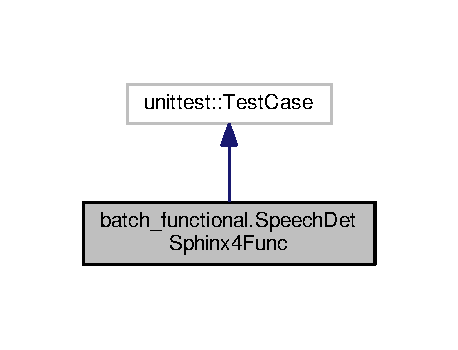
\includegraphics[width=220pt]{classbatch__functional_1_1SpeechDetSphinx4Func__inherit__graph}
\end{center}
\end{figure}


Collaboration diagram for batch\-\_\-functional.\-Speech\-Det\-Sphinx4\-Func\-:
\nopagebreak
\begin{figure}[H]
\begin{center}
\leavevmode
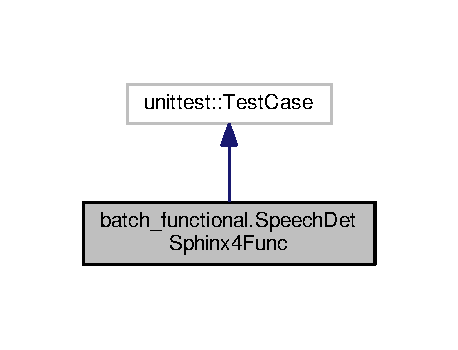
\includegraphics[width=220pt]{classbatch__functional_1_1SpeechDetSphinx4Func__coll__graph}
\end{center}
\end{figure}
\subsection*{Public Member Functions}
\begin{DoxyCompactItemize}
\item 
def \hyperlink{classbatch__functional_1_1SpeechDetSphinx4Func_a3c9455a650ec1a3d9a00633a77f8f3f5}{test\-\_\-batch\-Service}
\item 
def \hyperlink{classbatch__functional_1_1SpeechDetSphinx4Func_a316641ac7870ddb63490749b4792b590}{test\-\_\-batch\-Service1\-Ch}
\item 
def \hyperlink{classbatch__functional_1_1SpeechDetSphinx4Func_a4d12d3b504c8fc29e7c9b8e70cfeafeb}{test\-\_\-batch\-Service\-\_\-stress}
\item 
def \hyperlink{classbatch__functional_1_1SpeechDetSphinx4Func_a0c6afe405631c51df8d4a77b1dcb7948}{test\-\_\-batch\-Service\-Error\-Grammar}
\item 
def \hyperlink{classbatch__functional_1_1SpeechDetSphinx4Func_a6f945f6044e7ea87104b09ff78246c92}{test\-\_\-batch\-Service\-Error\-Language}
\item 
def \hyperlink{classbatch__functional_1_1SpeechDetSphinx4Func_addc7e5d430efa25e53a1f8b009fd3b27}{test\-\_\-batch\-Service\-Error\-Sentences}
\item 
def \hyperlink{classbatch__functional_1_1SpeechDetSphinx4Func_a60e1d7080a383403819714762985a711}{test\-\_\-batch\-Service\-Multilanguage}
\item 
def \hyperlink{classbatch__functional_1_1SpeechDetSphinx4Func_aa8ba2178adfc4b21cebbb4a6b5da150d}{test\-\_\-batch\-Service\-Ogg}
\item 
def \hyperlink{classbatch__functional_1_1SpeechDetSphinx4Func_ae2dd4750a0e80ea44031177010853800}{test\-\_\-batch\-Service\-Wrong\-File}
\item 
def \hyperlink{classbatch__functional_1_1SpeechDetSphinx4Func_a5e136352309b7a428b13ad668a4c765c}{test\-\_\-batch\-Service\-Wrong\-Type}
\item 
def \hyperlink{classbatch__functional_1_1SpeechDetSphinx4Func_ae5bbcb5d348b49172f0de8243f0dcb59}{test\-\_\-batch\-Service\-Wrong\-User}
\end{DoxyCompactItemize}


\subsection{Detailed Description}


Definition at line 38 of file batch\-\_\-functional.\-py.



\subsection{Member Function Documentation}
\hypertarget{classbatch__functional_1_1SpeechDetSphinx4Func_a3c9455a650ec1a3d9a00633a77f8f3f5}{\index{batch\-\_\-functional\-::\-Speech\-Det\-Sphinx4\-Func@{batch\-\_\-functional\-::\-Speech\-Det\-Sphinx4\-Func}!test\-\_\-batch\-Service@{test\-\_\-batch\-Service}}
\index{test\-\_\-batch\-Service@{test\-\_\-batch\-Service}!batch_functional::SpeechDetSphinx4Func@{batch\-\_\-functional\-::\-Speech\-Det\-Sphinx4\-Func}}
\subsubsection[{test\-\_\-batch\-Service}]{\setlength{\rightskip}{0pt plus 5cm}def batch\-\_\-functional.\-Speech\-Det\-Sphinx4\-Func.\-test\-\_\-batch\-Service (
\begin{DoxyParamCaption}
\item[{}]{self}
\end{DoxyParamCaption}
)}}\label{classbatch__functional_1_1SpeechDetSphinx4Func_a3c9455a650ec1a3d9a00633a77f8f3f5}


Definition at line 40 of file batch\-\_\-functional.\-py.

\hypertarget{classbatch__functional_1_1SpeechDetSphinx4Func_a316641ac7870ddb63490749b4792b590}{\index{batch\-\_\-functional\-::\-Speech\-Det\-Sphinx4\-Func@{batch\-\_\-functional\-::\-Speech\-Det\-Sphinx4\-Func}!test\-\_\-batch\-Service1\-Ch@{test\-\_\-batch\-Service1\-Ch}}
\index{test\-\_\-batch\-Service1\-Ch@{test\-\_\-batch\-Service1\-Ch}!batch_functional::SpeechDetSphinx4Func@{batch\-\_\-functional\-::\-Speech\-Det\-Sphinx4\-Func}}
\subsubsection[{test\-\_\-batch\-Service1\-Ch}]{\setlength{\rightskip}{0pt plus 5cm}def batch\-\_\-functional.\-Speech\-Det\-Sphinx4\-Func.\-test\-\_\-batch\-Service1\-Ch (
\begin{DoxyParamCaption}
\item[{}]{self}
\end{DoxyParamCaption}
)}}\label{classbatch__functional_1_1SpeechDetSphinx4Func_a316641ac7870ddb63490749b4792b590}


Definition at line 221 of file batch\-\_\-functional.\-py.

\hypertarget{classbatch__functional_1_1SpeechDetSphinx4Func_a4d12d3b504c8fc29e7c9b8e70cfeafeb}{\index{batch\-\_\-functional\-::\-Speech\-Det\-Sphinx4\-Func@{batch\-\_\-functional\-::\-Speech\-Det\-Sphinx4\-Func}!test\-\_\-batch\-Service\-\_\-stress@{test\-\_\-batch\-Service\-\_\-stress}}
\index{test\-\_\-batch\-Service\-\_\-stress@{test\-\_\-batch\-Service\-\_\-stress}!batch_functional::SpeechDetSphinx4Func@{batch\-\_\-functional\-::\-Speech\-Det\-Sphinx4\-Func}}
\subsubsection[{test\-\_\-batch\-Service\-\_\-stress}]{\setlength{\rightskip}{0pt plus 5cm}def batch\-\_\-functional.\-Speech\-Det\-Sphinx4\-Func.\-test\-\_\-batch\-Service\-\_\-stress (
\begin{DoxyParamCaption}
\item[{}]{self}
\end{DoxyParamCaption}
)}}\label{classbatch__functional_1_1SpeechDetSphinx4Func_a4d12d3b504c8fc29e7c9b8e70cfeafeb}


Definition at line 64 of file batch\-\_\-functional.\-py.

\hypertarget{classbatch__functional_1_1SpeechDetSphinx4Func_a0c6afe405631c51df8d4a77b1dcb7948}{\index{batch\-\_\-functional\-::\-Speech\-Det\-Sphinx4\-Func@{batch\-\_\-functional\-::\-Speech\-Det\-Sphinx4\-Func}!test\-\_\-batch\-Service\-Error\-Grammar@{test\-\_\-batch\-Service\-Error\-Grammar}}
\index{test\-\_\-batch\-Service\-Error\-Grammar@{test\-\_\-batch\-Service\-Error\-Grammar}!batch_functional::SpeechDetSphinx4Func@{batch\-\_\-functional\-::\-Speech\-Det\-Sphinx4\-Func}}
\subsubsection[{test\-\_\-batch\-Service\-Error\-Grammar}]{\setlength{\rightskip}{0pt plus 5cm}def batch\-\_\-functional.\-Speech\-Det\-Sphinx4\-Func.\-test\-\_\-batch\-Service\-Error\-Grammar (
\begin{DoxyParamCaption}
\item[{}]{self}
\end{DoxyParamCaption}
)}}\label{classbatch__functional_1_1SpeechDetSphinx4Func_a0c6afe405631c51df8d4a77b1dcb7948}


Definition at line 133 of file batch\-\_\-functional.\-py.

\hypertarget{classbatch__functional_1_1SpeechDetSphinx4Func_a6f945f6044e7ea87104b09ff78246c92}{\index{batch\-\_\-functional\-::\-Speech\-Det\-Sphinx4\-Func@{batch\-\_\-functional\-::\-Speech\-Det\-Sphinx4\-Func}!test\-\_\-batch\-Service\-Error\-Language@{test\-\_\-batch\-Service\-Error\-Language}}
\index{test\-\_\-batch\-Service\-Error\-Language@{test\-\_\-batch\-Service\-Error\-Language}!batch_functional::SpeechDetSphinx4Func@{batch\-\_\-functional\-::\-Speech\-Det\-Sphinx4\-Func}}
\subsubsection[{test\-\_\-batch\-Service\-Error\-Language}]{\setlength{\rightskip}{0pt plus 5cm}def batch\-\_\-functional.\-Speech\-Det\-Sphinx4\-Func.\-test\-\_\-batch\-Service\-Error\-Language (
\begin{DoxyParamCaption}
\item[{}]{self}
\end{DoxyParamCaption}
)}}\label{classbatch__functional_1_1SpeechDetSphinx4Func_a6f945f6044e7ea87104b09ff78246c92}


Definition at line 89 of file batch\-\_\-functional.\-py.

\hypertarget{classbatch__functional_1_1SpeechDetSphinx4Func_addc7e5d430efa25e53a1f8b009fd3b27}{\index{batch\-\_\-functional\-::\-Speech\-Det\-Sphinx4\-Func@{batch\-\_\-functional\-::\-Speech\-Det\-Sphinx4\-Func}!test\-\_\-batch\-Service\-Error\-Sentences@{test\-\_\-batch\-Service\-Error\-Sentences}}
\index{test\-\_\-batch\-Service\-Error\-Sentences@{test\-\_\-batch\-Service\-Error\-Sentences}!batch_functional::SpeechDetSphinx4Func@{batch\-\_\-functional\-::\-Speech\-Det\-Sphinx4\-Func}}
\subsubsection[{test\-\_\-batch\-Service\-Error\-Sentences}]{\setlength{\rightskip}{0pt plus 5cm}def batch\-\_\-functional.\-Speech\-Det\-Sphinx4\-Func.\-test\-\_\-batch\-Service\-Error\-Sentences (
\begin{DoxyParamCaption}
\item[{}]{self}
\end{DoxyParamCaption}
)}}\label{classbatch__functional_1_1SpeechDetSphinx4Func_addc7e5d430efa25e53a1f8b009fd3b27}


Definition at line 111 of file batch\-\_\-functional.\-py.

\hypertarget{classbatch__functional_1_1SpeechDetSphinx4Func_a60e1d7080a383403819714762985a711}{\index{batch\-\_\-functional\-::\-Speech\-Det\-Sphinx4\-Func@{batch\-\_\-functional\-::\-Speech\-Det\-Sphinx4\-Func}!test\-\_\-batch\-Service\-Multilanguage@{test\-\_\-batch\-Service\-Multilanguage}}
\index{test\-\_\-batch\-Service\-Multilanguage@{test\-\_\-batch\-Service\-Multilanguage}!batch_functional::SpeechDetSphinx4Func@{batch\-\_\-functional\-::\-Speech\-Det\-Sphinx4\-Func}}
\subsubsection[{test\-\_\-batch\-Service\-Multilanguage}]{\setlength{\rightskip}{0pt plus 5cm}def batch\-\_\-functional.\-Speech\-Det\-Sphinx4\-Func.\-test\-\_\-batch\-Service\-Multilanguage (
\begin{DoxyParamCaption}
\item[{}]{self}
\end{DoxyParamCaption}
)}}\label{classbatch__functional_1_1SpeechDetSphinx4Func_a60e1d7080a383403819714762985a711}


Definition at line 268 of file batch\-\_\-functional.\-py.

\hypertarget{classbatch__functional_1_1SpeechDetSphinx4Func_aa8ba2178adfc4b21cebbb4a6b5da150d}{\index{batch\-\_\-functional\-::\-Speech\-Det\-Sphinx4\-Func@{batch\-\_\-functional\-::\-Speech\-Det\-Sphinx4\-Func}!test\-\_\-batch\-Service\-Ogg@{test\-\_\-batch\-Service\-Ogg}}
\index{test\-\_\-batch\-Service\-Ogg@{test\-\_\-batch\-Service\-Ogg}!batch_functional::SpeechDetSphinx4Func@{batch\-\_\-functional\-::\-Speech\-Det\-Sphinx4\-Func}}
\subsubsection[{test\-\_\-batch\-Service\-Ogg}]{\setlength{\rightskip}{0pt plus 5cm}def batch\-\_\-functional.\-Speech\-Det\-Sphinx4\-Func.\-test\-\_\-batch\-Service\-Ogg (
\begin{DoxyParamCaption}
\item[{}]{self}
\end{DoxyParamCaption}
)}}\label{classbatch__functional_1_1SpeechDetSphinx4Func_aa8ba2178adfc4b21cebbb4a6b5da150d}


Definition at line 244 of file batch\-\_\-functional.\-py.

\hypertarget{classbatch__functional_1_1SpeechDetSphinx4Func_ae2dd4750a0e80ea44031177010853800}{\index{batch\-\_\-functional\-::\-Speech\-Det\-Sphinx4\-Func@{batch\-\_\-functional\-::\-Speech\-Det\-Sphinx4\-Func}!test\-\_\-batch\-Service\-Wrong\-File@{test\-\_\-batch\-Service\-Wrong\-File}}
\index{test\-\_\-batch\-Service\-Wrong\-File@{test\-\_\-batch\-Service\-Wrong\-File}!batch_functional::SpeechDetSphinx4Func@{batch\-\_\-functional\-::\-Speech\-Det\-Sphinx4\-Func}}
\subsubsection[{test\-\_\-batch\-Service\-Wrong\-File}]{\setlength{\rightskip}{0pt plus 5cm}def batch\-\_\-functional.\-Speech\-Det\-Sphinx4\-Func.\-test\-\_\-batch\-Service\-Wrong\-File (
\begin{DoxyParamCaption}
\item[{}]{self}
\end{DoxyParamCaption}
)}}\label{classbatch__functional_1_1SpeechDetSphinx4Func_ae2dd4750a0e80ea44031177010853800}


Definition at line 155 of file batch\-\_\-functional.\-py.

\hypertarget{classbatch__functional_1_1SpeechDetSphinx4Func_a5e136352309b7a428b13ad668a4c765c}{\index{batch\-\_\-functional\-::\-Speech\-Det\-Sphinx4\-Func@{batch\-\_\-functional\-::\-Speech\-Det\-Sphinx4\-Func}!test\-\_\-batch\-Service\-Wrong\-Type@{test\-\_\-batch\-Service\-Wrong\-Type}}
\index{test\-\_\-batch\-Service\-Wrong\-Type@{test\-\_\-batch\-Service\-Wrong\-Type}!batch_functional::SpeechDetSphinx4Func@{batch\-\_\-functional\-::\-Speech\-Det\-Sphinx4\-Func}}
\subsubsection[{test\-\_\-batch\-Service\-Wrong\-Type}]{\setlength{\rightskip}{0pt plus 5cm}def batch\-\_\-functional.\-Speech\-Det\-Sphinx4\-Func.\-test\-\_\-batch\-Service\-Wrong\-Type (
\begin{DoxyParamCaption}
\item[{}]{self}
\end{DoxyParamCaption}
)}}\label{classbatch__functional_1_1SpeechDetSphinx4Func_a5e136352309b7a428b13ad668a4c765c}


Definition at line 199 of file batch\-\_\-functional.\-py.

\hypertarget{classbatch__functional_1_1SpeechDetSphinx4Func_ae5bbcb5d348b49172f0de8243f0dcb59}{\index{batch\-\_\-functional\-::\-Speech\-Det\-Sphinx4\-Func@{batch\-\_\-functional\-::\-Speech\-Det\-Sphinx4\-Func}!test\-\_\-batch\-Service\-Wrong\-User@{test\-\_\-batch\-Service\-Wrong\-User}}
\index{test\-\_\-batch\-Service\-Wrong\-User@{test\-\_\-batch\-Service\-Wrong\-User}!batch_functional::SpeechDetSphinx4Func@{batch\-\_\-functional\-::\-Speech\-Det\-Sphinx4\-Func}}
\subsubsection[{test\-\_\-batch\-Service\-Wrong\-User}]{\setlength{\rightskip}{0pt plus 5cm}def batch\-\_\-functional.\-Speech\-Det\-Sphinx4\-Func.\-test\-\_\-batch\-Service\-Wrong\-User (
\begin{DoxyParamCaption}
\item[{}]{self}
\end{DoxyParamCaption}
)}}\label{classbatch__functional_1_1SpeechDetSphinx4Func_ae5bbcb5d348b49172f0de8243f0dcb59}


Definition at line 177 of file batch\-\_\-functional.\-py.



The documentation for this class was generated from the following file\-:\begin{DoxyCompactItemize}
\item 
/home/travis/rapp\-\_\-temp/rapp-\/platform/rapp\-\_\-speech\-\_\-detection\-\_\-sphinx4/tests/functional/\hyperlink{batch__functional_8py}{batch\-\_\-functional.\-py}\end{DoxyCompactItemize}

\hypertarget{classenglish__support__unit__tests_1_1TestAudioProcessing}{\section{english\-\_\-support\-\_\-unit\-\_\-tests.\-Test\-Audio\-Processing Class Reference}
\label{classenglish__support__unit__tests_1_1TestAudioProcessing}\index{english\-\_\-support\-\_\-unit\-\_\-tests.\-Test\-Audio\-Processing@{english\-\_\-support\-\_\-unit\-\_\-tests.\-Test\-Audio\-Processing}}
}


Inheritance diagram for english\-\_\-support\-\_\-unit\-\_\-tests.\-Test\-Audio\-Processing\-:
\nopagebreak
\begin{figure}[H]
\begin{center}
\leavevmode
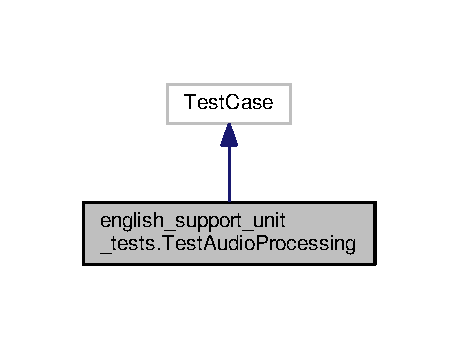
\includegraphics[width=220pt]{classenglish__support__unit__tests_1_1TestAudioProcessing__inherit__graph}
\end{center}
\end{figure}


Collaboration diagram for english\-\_\-support\-\_\-unit\-\_\-tests.\-Test\-Audio\-Processing\-:
\nopagebreak
\begin{figure}[H]
\begin{center}
\leavevmode
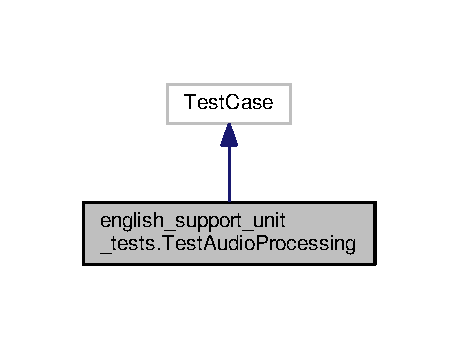
\includegraphics[width=220pt]{classenglish__support__unit__tests_1_1TestAudioProcessing__coll__graph}
\end{center}
\end{figure}
\subsection*{Public Member Functions}
\begin{DoxyCompactItemize}
\item 
def \hyperlink{classenglish__support__unit__tests_1_1TestAudioProcessing_a0c4275044a58bff1192579b87c86f71c}{set\-Up}
\item 
def \hyperlink{classenglish__support__unit__tests_1_1TestAudioProcessing_abddf049b5dbfd26903167694abab5506}{tear\-Down}
\item 
def \hyperlink{classenglish__support__unit__tests_1_1TestAudioProcessing_a49fe0076ebda8e012abf9e79d28b4049}{test\-\_\-generic\-Configuration\-Files}
\item 
def \hyperlink{classenglish__support__unit__tests_1_1TestAudioProcessing_aac1fc989bb8c79cf941f54febabe3f39}{test\-\_\-limited\-Vocabulary\-Configuration\-Files\-\_\-correct\-Case}
\item 
def \hyperlink{classenglish__support__unit__tests_1_1TestAudioProcessing_a0baa86921674f6631da9ac2c13f1d0ed}{test\-\_\-limited\-Vocabulary\-Configuration\-Files\-\_\-not\-Existent\-Words}
\end{DoxyCompactItemize}
\subsection*{Public Attributes}
\begin{DoxyCompactItemize}
\item 
\hyperlink{classenglish__support__unit__tests_1_1TestAudioProcessing_a382b4b85899f9b39d213de0ba1ab85d2}{english\-\_\-support\-\_\-module}
\item 
\hyperlink{classenglish__support__unit__tests_1_1TestAudioProcessing_a107b29275347e41f4d9b65d3934b0188}{utilities\-\_\-module}
\end{DoxyCompactItemize}


\subsection{Detailed Description}


Definition at line 27 of file english\-\_\-support\-\_\-unit\-\_\-tests.\-py.



\subsection{Member Function Documentation}
\hypertarget{classenglish__support__unit__tests_1_1TestAudioProcessing_a0c4275044a58bff1192579b87c86f71c}{\index{english\-\_\-support\-\_\-unit\-\_\-tests\-::\-Test\-Audio\-Processing@{english\-\_\-support\-\_\-unit\-\_\-tests\-::\-Test\-Audio\-Processing}!set\-Up@{set\-Up}}
\index{set\-Up@{set\-Up}!english_support_unit_tests::TestAudioProcessing@{english\-\_\-support\-\_\-unit\-\_\-tests\-::\-Test\-Audio\-Processing}}
\subsubsection[{set\-Up}]{\setlength{\rightskip}{0pt plus 5cm}def english\-\_\-support\-\_\-unit\-\_\-tests.\-Test\-Audio\-Processing.\-set\-Up (
\begin{DoxyParamCaption}
\item[{}]{self}
\end{DoxyParamCaption}
)}}\label{classenglish__support__unit__tests_1_1TestAudioProcessing_a0c4275044a58bff1192579b87c86f71c}


Definition at line 28 of file english\-\_\-support\-\_\-unit\-\_\-tests.\-py.

\hypertarget{classenglish__support__unit__tests_1_1TestAudioProcessing_abddf049b5dbfd26903167694abab5506}{\index{english\-\_\-support\-\_\-unit\-\_\-tests\-::\-Test\-Audio\-Processing@{english\-\_\-support\-\_\-unit\-\_\-tests\-::\-Test\-Audio\-Processing}!tear\-Down@{tear\-Down}}
\index{tear\-Down@{tear\-Down}!english_support_unit_tests::TestAudioProcessing@{english\-\_\-support\-\_\-unit\-\_\-tests\-::\-Test\-Audio\-Processing}}
\subsubsection[{tear\-Down}]{\setlength{\rightskip}{0pt plus 5cm}def english\-\_\-support\-\_\-unit\-\_\-tests.\-Test\-Audio\-Processing.\-tear\-Down (
\begin{DoxyParamCaption}
\item[{}]{self}
\end{DoxyParamCaption}
)}}\label{classenglish__support__unit__tests_1_1TestAudioProcessing_abddf049b5dbfd26903167694abab5506}


Definition at line 31 of file english\-\_\-support\-\_\-unit\-\_\-tests.\-py.

\hypertarget{classenglish__support__unit__tests_1_1TestAudioProcessing_a49fe0076ebda8e012abf9e79d28b4049}{\index{english\-\_\-support\-\_\-unit\-\_\-tests\-::\-Test\-Audio\-Processing@{english\-\_\-support\-\_\-unit\-\_\-tests\-::\-Test\-Audio\-Processing}!test\-\_\-generic\-Configuration\-Files@{test\-\_\-generic\-Configuration\-Files}}
\index{test\-\_\-generic\-Configuration\-Files@{test\-\_\-generic\-Configuration\-Files}!english_support_unit_tests::TestAudioProcessing@{english\-\_\-support\-\_\-unit\-\_\-tests\-::\-Test\-Audio\-Processing}}
\subsubsection[{test\-\_\-generic\-Configuration\-Files}]{\setlength{\rightskip}{0pt plus 5cm}def english\-\_\-support\-\_\-unit\-\_\-tests.\-Test\-Audio\-Processing.\-test\-\_\-generic\-Configuration\-Files (
\begin{DoxyParamCaption}
\item[{}]{self}
\end{DoxyParamCaption}
)}}\label{classenglish__support__unit__tests_1_1TestAudioProcessing_a49fe0076ebda8e012abf9e79d28b4049}


Definition at line 34 of file english\-\_\-support\-\_\-unit\-\_\-tests.\-py.

\hypertarget{classenglish__support__unit__tests_1_1TestAudioProcessing_aac1fc989bb8c79cf941f54febabe3f39}{\index{english\-\_\-support\-\_\-unit\-\_\-tests\-::\-Test\-Audio\-Processing@{english\-\_\-support\-\_\-unit\-\_\-tests\-::\-Test\-Audio\-Processing}!test\-\_\-limited\-Vocabulary\-Configuration\-Files\-\_\-correct\-Case@{test\-\_\-limited\-Vocabulary\-Configuration\-Files\-\_\-correct\-Case}}
\index{test\-\_\-limited\-Vocabulary\-Configuration\-Files\-\_\-correct\-Case@{test\-\_\-limited\-Vocabulary\-Configuration\-Files\-\_\-correct\-Case}!english_support_unit_tests::TestAudioProcessing@{english\-\_\-support\-\_\-unit\-\_\-tests\-::\-Test\-Audio\-Processing}}
\subsubsection[{test\-\_\-limited\-Vocabulary\-Configuration\-Files\-\_\-correct\-Case}]{\setlength{\rightskip}{0pt plus 5cm}def english\-\_\-support\-\_\-unit\-\_\-tests.\-Test\-Audio\-Processing.\-test\-\_\-limited\-Vocabulary\-Configuration\-Files\-\_\-correct\-Case (
\begin{DoxyParamCaption}
\item[{}]{self}
\end{DoxyParamCaption}
)}}\label{classenglish__support__unit__tests_1_1TestAudioProcessing_aac1fc989bb8c79cf941f54febabe3f39}


Definition at line 58 of file english\-\_\-support\-\_\-unit\-\_\-tests.\-py.

\hypertarget{classenglish__support__unit__tests_1_1TestAudioProcessing_a0baa86921674f6631da9ac2c13f1d0ed}{\index{english\-\_\-support\-\_\-unit\-\_\-tests\-::\-Test\-Audio\-Processing@{english\-\_\-support\-\_\-unit\-\_\-tests\-::\-Test\-Audio\-Processing}!test\-\_\-limited\-Vocabulary\-Configuration\-Files\-\_\-not\-Existent\-Words@{test\-\_\-limited\-Vocabulary\-Configuration\-Files\-\_\-not\-Existent\-Words}}
\index{test\-\_\-limited\-Vocabulary\-Configuration\-Files\-\_\-not\-Existent\-Words@{test\-\_\-limited\-Vocabulary\-Configuration\-Files\-\_\-not\-Existent\-Words}!english_support_unit_tests::TestAudioProcessing@{english\-\_\-support\-\_\-unit\-\_\-tests\-::\-Test\-Audio\-Processing}}
\subsubsection[{test\-\_\-limited\-Vocabulary\-Configuration\-Files\-\_\-not\-Existent\-Words}]{\setlength{\rightskip}{0pt plus 5cm}def english\-\_\-support\-\_\-unit\-\_\-tests.\-Test\-Audio\-Processing.\-test\-\_\-limited\-Vocabulary\-Configuration\-Files\-\_\-not\-Existent\-Words (
\begin{DoxyParamCaption}
\item[{}]{self}
\end{DoxyParamCaption}
)}}\label{classenglish__support__unit__tests_1_1TestAudioProcessing_a0baa86921674f6631da9ac2c13f1d0ed}


Definition at line 88 of file english\-\_\-support\-\_\-unit\-\_\-tests.\-py.



\subsection{Member Data Documentation}
\hypertarget{classenglish__support__unit__tests_1_1TestAudioProcessing_a382b4b85899f9b39d213de0ba1ab85d2}{\index{english\-\_\-support\-\_\-unit\-\_\-tests\-::\-Test\-Audio\-Processing@{english\-\_\-support\-\_\-unit\-\_\-tests\-::\-Test\-Audio\-Processing}!english\-\_\-support\-\_\-module@{english\-\_\-support\-\_\-module}}
\index{english\-\_\-support\-\_\-module@{english\-\_\-support\-\_\-module}!english_support_unit_tests::TestAudioProcessing@{english\-\_\-support\-\_\-unit\-\_\-tests\-::\-Test\-Audio\-Processing}}
\subsubsection[{english\-\_\-support\-\_\-module}]{\setlength{\rightskip}{0pt plus 5cm}english\-\_\-support\-\_\-unit\-\_\-tests.\-Test\-Audio\-Processing.\-english\-\_\-support\-\_\-module}}\label{classenglish__support__unit__tests_1_1TestAudioProcessing_a382b4b85899f9b39d213de0ba1ab85d2}


Definition at line 29 of file english\-\_\-support\-\_\-unit\-\_\-tests.\-py.

\hypertarget{classenglish__support__unit__tests_1_1TestAudioProcessing_a107b29275347e41f4d9b65d3934b0188}{\index{english\-\_\-support\-\_\-unit\-\_\-tests\-::\-Test\-Audio\-Processing@{english\-\_\-support\-\_\-unit\-\_\-tests\-::\-Test\-Audio\-Processing}!utilities\-\_\-module@{utilities\-\_\-module}}
\index{utilities\-\_\-module@{utilities\-\_\-module}!english_support_unit_tests::TestAudioProcessing@{english\-\_\-support\-\_\-unit\-\_\-tests\-::\-Test\-Audio\-Processing}}
\subsubsection[{utilities\-\_\-module}]{\setlength{\rightskip}{0pt plus 5cm}english\-\_\-support\-\_\-unit\-\_\-tests.\-Test\-Audio\-Processing.\-utilities\-\_\-module}}\label{classenglish__support__unit__tests_1_1TestAudioProcessing_a107b29275347e41f4d9b65d3934b0188}


Definition at line 32 of file english\-\_\-support\-\_\-unit\-\_\-tests.\-py.



The documentation for this class was generated from the following file\-:\begin{DoxyCompactItemize}
\item 
/home/travis/rapp\-\_\-temp/rapp-\/platform/rapp\-\_\-speech\-\_\-detection\-\_\-sphinx4/tests/unit/\hyperlink{english__support__unit__tests_8py}{english\-\_\-support\-\_\-unit\-\_\-tests.\-py}\end{DoxyCompactItemize}

\hypertarget{classlimited__vocabulary__creator__unit__tests_1_1TestAudioProcessing}{\section{limited\-\_\-vocabulary\-\_\-creator\-\_\-unit\-\_\-tests.\-Test\-Audio\-Processing Class Reference}
\label{classlimited__vocabulary__creator__unit__tests_1_1TestAudioProcessing}\index{limited\-\_\-vocabulary\-\_\-creator\-\_\-unit\-\_\-tests.\-Test\-Audio\-Processing@{limited\-\_\-vocabulary\-\_\-creator\-\_\-unit\-\_\-tests.\-Test\-Audio\-Processing}}
}


Inheritance diagram for limited\-\_\-vocabulary\-\_\-creator\-\_\-unit\-\_\-tests.\-Test\-Audio\-Processing\-:


Collaboration diagram for limited\-\_\-vocabulary\-\_\-creator\-\_\-unit\-\_\-tests.\-Test\-Audio\-Processing\-:
\subsection*{Public Member Functions}
\begin{DoxyCompactItemize}
\item 
def \hyperlink{classlimited__vocabulary__creator__unit__tests_1_1TestAudioProcessing_a7d117106303f6b37caa92222f38a547b}{set\-Up}
\item 
def \hyperlink{classlimited__vocabulary__creator__unit__tests_1_1TestAudioProcessing_ac0e1025eba3f01c3ea857bfaa8c67ee5}{tear\-Down}
\item 
def \hyperlink{classlimited__vocabulary__creator__unit__tests_1_1TestAudioProcessing_aa02d8e6e8cc2eb4944d23065b1f61a29}{test\-\_\-normal\-Case}
\item 
def \hyperlink{classlimited__vocabulary__creator__unit__tests_1_1TestAudioProcessing_a558b72f2e42b4ded6b90ca51ab64f925}{test\-\_\-no\-Sentences}
\end{DoxyCompactItemize}
\subsection*{Public Attributes}
\begin{DoxyCompactItemize}
\item 
\hyperlink{classlimited__vocabulary__creator__unit__tests_1_1TestAudioProcessing_a3a245e4b4de98cee967b701ada399354}{module}
\end{DoxyCompactItemize}


\subsection{Detailed Description}


Definition at line 27 of file limited\-\_\-vocabulary\-\_\-creator\-\_\-unit\-\_\-tests.\-py.



\subsection{Member Function Documentation}
\hypertarget{classlimited__vocabulary__creator__unit__tests_1_1TestAudioProcessing_a7d117106303f6b37caa92222f38a547b}{\index{limited\-\_\-vocabulary\-\_\-creator\-\_\-unit\-\_\-tests\-::\-Test\-Audio\-Processing@{limited\-\_\-vocabulary\-\_\-creator\-\_\-unit\-\_\-tests\-::\-Test\-Audio\-Processing}!set\-Up@{set\-Up}}
\index{set\-Up@{set\-Up}!limited_vocabulary_creator_unit_tests::TestAudioProcessing@{limited\-\_\-vocabulary\-\_\-creator\-\_\-unit\-\_\-tests\-::\-Test\-Audio\-Processing}}
\subsubsection[{set\-Up}]{\setlength{\rightskip}{0pt plus 5cm}def limited\-\_\-vocabulary\-\_\-creator\-\_\-unit\-\_\-tests.\-Test\-Audio\-Processing.\-set\-Up (
\begin{DoxyParamCaption}
\item[{}]{self}
\end{DoxyParamCaption}
)}}\label{classlimited__vocabulary__creator__unit__tests_1_1TestAudioProcessing_a7d117106303f6b37caa92222f38a547b}


Definition at line 28 of file limited\-\_\-vocabulary\-\_\-creator\-\_\-unit\-\_\-tests.\-py.

\hypertarget{classlimited__vocabulary__creator__unit__tests_1_1TestAudioProcessing_ac0e1025eba3f01c3ea857bfaa8c67ee5}{\index{limited\-\_\-vocabulary\-\_\-creator\-\_\-unit\-\_\-tests\-::\-Test\-Audio\-Processing@{limited\-\_\-vocabulary\-\_\-creator\-\_\-unit\-\_\-tests\-::\-Test\-Audio\-Processing}!tear\-Down@{tear\-Down}}
\index{tear\-Down@{tear\-Down}!limited_vocabulary_creator_unit_tests::TestAudioProcessing@{limited\-\_\-vocabulary\-\_\-creator\-\_\-unit\-\_\-tests\-::\-Test\-Audio\-Processing}}
\subsubsection[{tear\-Down}]{\setlength{\rightskip}{0pt plus 5cm}def limited\-\_\-vocabulary\-\_\-creator\-\_\-unit\-\_\-tests.\-Test\-Audio\-Processing.\-tear\-Down (
\begin{DoxyParamCaption}
\item[{}]{self}
\end{DoxyParamCaption}
)}}\label{classlimited__vocabulary__creator__unit__tests_1_1TestAudioProcessing_ac0e1025eba3f01c3ea857bfaa8c67ee5}


Definition at line 31 of file limited\-\_\-vocabulary\-\_\-creator\-\_\-unit\-\_\-tests.\-py.

\hypertarget{classlimited__vocabulary__creator__unit__tests_1_1TestAudioProcessing_aa02d8e6e8cc2eb4944d23065b1f61a29}{\index{limited\-\_\-vocabulary\-\_\-creator\-\_\-unit\-\_\-tests\-::\-Test\-Audio\-Processing@{limited\-\_\-vocabulary\-\_\-creator\-\_\-unit\-\_\-tests\-::\-Test\-Audio\-Processing}!test\-\_\-normal\-Case@{test\-\_\-normal\-Case}}
\index{test\-\_\-normal\-Case@{test\-\_\-normal\-Case}!limited_vocabulary_creator_unit_tests::TestAudioProcessing@{limited\-\_\-vocabulary\-\_\-creator\-\_\-unit\-\_\-tests\-::\-Test\-Audio\-Processing}}
\subsubsection[{test\-\_\-normal\-Case}]{\setlength{\rightskip}{0pt plus 5cm}def limited\-\_\-vocabulary\-\_\-creator\-\_\-unit\-\_\-tests.\-Test\-Audio\-Processing.\-test\-\_\-normal\-Case (
\begin{DoxyParamCaption}
\item[{}]{self}
\end{DoxyParamCaption}
)}}\label{classlimited__vocabulary__creator__unit__tests_1_1TestAudioProcessing_aa02d8e6e8cc2eb4944d23065b1f61a29}


Definition at line 34 of file limited\-\_\-vocabulary\-\_\-creator\-\_\-unit\-\_\-tests.\-py.

\hypertarget{classlimited__vocabulary__creator__unit__tests_1_1TestAudioProcessing_a558b72f2e42b4ded6b90ca51ab64f925}{\index{limited\-\_\-vocabulary\-\_\-creator\-\_\-unit\-\_\-tests\-::\-Test\-Audio\-Processing@{limited\-\_\-vocabulary\-\_\-creator\-\_\-unit\-\_\-tests\-::\-Test\-Audio\-Processing}!test\-\_\-no\-Sentences@{test\-\_\-no\-Sentences}}
\index{test\-\_\-no\-Sentences@{test\-\_\-no\-Sentences}!limited_vocabulary_creator_unit_tests::TestAudioProcessing@{limited\-\_\-vocabulary\-\_\-creator\-\_\-unit\-\_\-tests\-::\-Test\-Audio\-Processing}}
\subsubsection[{test\-\_\-no\-Sentences}]{\setlength{\rightskip}{0pt plus 5cm}def limited\-\_\-vocabulary\-\_\-creator\-\_\-unit\-\_\-tests.\-Test\-Audio\-Processing.\-test\-\_\-no\-Sentences (
\begin{DoxyParamCaption}
\item[{}]{self}
\end{DoxyParamCaption}
)}}\label{classlimited__vocabulary__creator__unit__tests_1_1TestAudioProcessing_a558b72f2e42b4ded6b90ca51ab64f925}


Definition at line 97 of file limited\-\_\-vocabulary\-\_\-creator\-\_\-unit\-\_\-tests.\-py.



\subsection{Member Data Documentation}
\hypertarget{classlimited__vocabulary__creator__unit__tests_1_1TestAudioProcessing_a3a245e4b4de98cee967b701ada399354}{\index{limited\-\_\-vocabulary\-\_\-creator\-\_\-unit\-\_\-tests\-::\-Test\-Audio\-Processing@{limited\-\_\-vocabulary\-\_\-creator\-\_\-unit\-\_\-tests\-::\-Test\-Audio\-Processing}!module@{module}}
\index{module@{module}!limited_vocabulary_creator_unit_tests::TestAudioProcessing@{limited\-\_\-vocabulary\-\_\-creator\-\_\-unit\-\_\-tests\-::\-Test\-Audio\-Processing}}
\subsubsection[{module}]{\setlength{\rightskip}{0pt plus 5cm}limited\-\_\-vocabulary\-\_\-creator\-\_\-unit\-\_\-tests.\-Test\-Audio\-Processing.\-module}}\label{classlimited__vocabulary__creator__unit__tests_1_1TestAudioProcessing_a3a245e4b4de98cee967b701ada399354}


Definition at line 29 of file limited\-\_\-vocabulary\-\_\-creator\-\_\-unit\-\_\-tests.\-py.



The documentation for this class was generated from the following file\-:\begin{DoxyCompactItemize}
\item 
/home/travis/rapp\-\_\-temp/rapp-\/platform/rapp\-\_\-speech\-\_\-detection\-\_\-sphinx4/tests/unit/\hyperlink{limited__vocabulary__creator__unit__tests_8py}{limited\-\_\-vocabulary\-\_\-creator\-\_\-unit\-\_\-tests.\-py}\end{DoxyCompactItemize}

\hypertarget{classgreek__support__unit__tests_1_1TestAudioProcessing}{\section{greek\-\_\-support\-\_\-unit\-\_\-tests.\-Test\-Audio\-Processing Class Reference}
\label{classgreek__support__unit__tests_1_1TestAudioProcessing}\index{greek\-\_\-support\-\_\-unit\-\_\-tests.\-Test\-Audio\-Processing@{greek\-\_\-support\-\_\-unit\-\_\-tests.\-Test\-Audio\-Processing}}
}


Inheritance diagram for greek\-\_\-support\-\_\-unit\-\_\-tests.\-Test\-Audio\-Processing\-:
\nopagebreak
\begin{figure}[H]
\begin{center}
\leavevmode
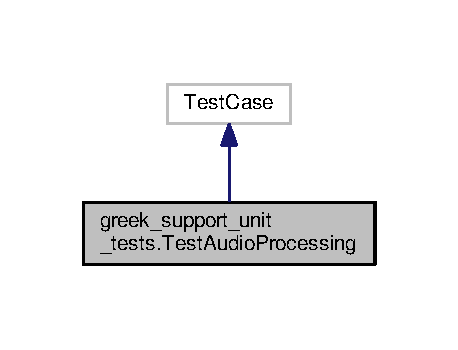
\includegraphics[width=220pt]{classgreek__support__unit__tests_1_1TestAudioProcessing__inherit__graph}
\end{center}
\end{figure}


Collaboration diagram for greek\-\_\-support\-\_\-unit\-\_\-tests.\-Test\-Audio\-Processing\-:
\nopagebreak
\begin{figure}[H]
\begin{center}
\leavevmode
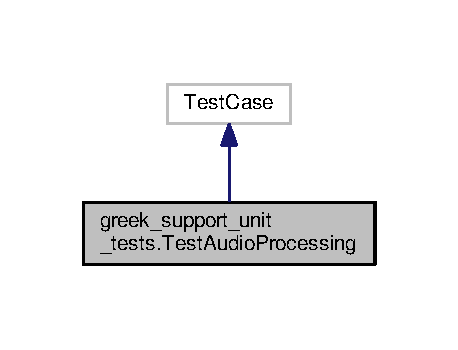
\includegraphics[width=220pt]{classgreek__support__unit__tests_1_1TestAudioProcessing__coll__graph}
\end{center}
\end{figure}
\subsection*{Public Member Functions}
\begin{DoxyCompactItemize}
\item 
def \hyperlink{classgreek__support__unit__tests_1_1TestAudioProcessing_a235dfd8fbbba93a77b341ebf8d7fb44f}{set\-Up}
\item 
def \hyperlink{classgreek__support__unit__tests_1_1TestAudioProcessing_a412e0172ba6255e53dd93b8499e0ae6f}{tear\-Down}
\item 
def \hyperlink{classgreek__support__unit__tests_1_1TestAudioProcessing_accc68064811fbf07a0602bfe4cbef643}{test\-\_\-transform\-Words\-\_\-case\-\_\-augo}
\item 
def \hyperlink{classgreek__support__unit__tests_1_1TestAudioProcessing_a3fcb700842d6d592f3b8b17fbff14eb7}{test\-\_\-transform\-Words\-\_\-case\-\_\-autos}
\item 
def \hyperlink{classgreek__support__unit__tests_1_1TestAudioProcessing_ab2c5d249fc9c76099d912aa38473da6d}{test\-\_\-transform\-Words\-\_\-case\-\_\-diairesi}
\item 
def \hyperlink{classgreek__support__unit__tests_1_1TestAudioProcessing_a33b4e7e80a4d51dd1a110a9168f0134c}{test\-\_\-transform\-Words\-\_\-case\-\_\-efstoxos}
\item 
def \hyperlink{classgreek__support__unit__tests_1_1TestAudioProcessing_a73f0bbc7b7398f3bfde28db3a8b1085f}{test\-\_\-transform\-Words\-\_\-case\-\_\-epistimonas}
\item 
def \hyperlink{classgreek__support__unit__tests_1_1TestAudioProcessing_a5e9e5337ec1de418f16ba04acb7d1195}{test\-\_\-transform\-Words\-\_\-case\-\_\-euxaristw}
\item 
def \hyperlink{classgreek__support__unit__tests_1_1TestAudioProcessing_a3b50e7709fbb7b7da7ab8480cca54f90}{test\-\_\-transform\-Words\-\_\-case\-\_\-exairetika}
\item 
def \hyperlink{classgreek__support__unit__tests_1_1TestAudioProcessing_a56bb0a110961ac313238583ac0a9456b}{test\-\_\-transform\-Words\-\_\-case\-\_\-kalytereyw}
\item 
def \hyperlink{classgreek__support__unit__tests_1_1TestAudioProcessing_a0edd822483fc91718e6dec07c86f6df8}{test\-\_\-transform\-Words\-\_\-case\-\_\-mallon}
\item 
def \hyperlink{classgreek__support__unit__tests_1_1TestAudioProcessing_a32eee319e08aab6a4414c688536494c7}{test\-\_\-transform\-Words\-\_\-case\-\_\-poini}
\item 
def \hyperlink{classgreek__support__unit__tests_1_1TestAudioProcessing_a781e2f5b661dc058cdc9c6ad129d0332}{test\-\_\-transform\-Words\-\_\-case\-\_\-wriaios}
\item 
def \hyperlink{classgreek__support__unit__tests_1_1TestAudioProcessing_a994d5c8dcfd668c5577a396454af1529}{test\-\_\-transform\-Words\-\_\-case\-\_\-xasma}
\end{DoxyCompactItemize}
\subsection*{Public Attributes}
\begin{DoxyCompactItemize}
\item 
\hyperlink{classgreek__support__unit__tests_1_1TestAudioProcessing_a82141fa5a1b98c4de7264f806c942fcd}{module}
\end{DoxyCompactItemize}


\subsection{Detailed Description}


Definition at line 27 of file greek\-\_\-support\-\_\-unit\-\_\-tests.\-py.



\subsection{Member Function Documentation}
\hypertarget{classgreek__support__unit__tests_1_1TestAudioProcessing_a235dfd8fbbba93a77b341ebf8d7fb44f}{\index{greek\-\_\-support\-\_\-unit\-\_\-tests\-::\-Test\-Audio\-Processing@{greek\-\_\-support\-\_\-unit\-\_\-tests\-::\-Test\-Audio\-Processing}!set\-Up@{set\-Up}}
\index{set\-Up@{set\-Up}!greek_support_unit_tests::TestAudioProcessing@{greek\-\_\-support\-\_\-unit\-\_\-tests\-::\-Test\-Audio\-Processing}}
\subsubsection[{set\-Up}]{\setlength{\rightskip}{0pt plus 5cm}def greek\-\_\-support\-\_\-unit\-\_\-tests.\-Test\-Audio\-Processing.\-set\-Up (
\begin{DoxyParamCaption}
\item[{}]{self}
\end{DoxyParamCaption}
)}}\label{classgreek__support__unit__tests_1_1TestAudioProcessing_a235dfd8fbbba93a77b341ebf8d7fb44f}


Definition at line 28 of file greek\-\_\-support\-\_\-unit\-\_\-tests.\-py.

\hypertarget{classgreek__support__unit__tests_1_1TestAudioProcessing_a412e0172ba6255e53dd93b8499e0ae6f}{\index{greek\-\_\-support\-\_\-unit\-\_\-tests\-::\-Test\-Audio\-Processing@{greek\-\_\-support\-\_\-unit\-\_\-tests\-::\-Test\-Audio\-Processing}!tear\-Down@{tear\-Down}}
\index{tear\-Down@{tear\-Down}!greek_support_unit_tests::TestAudioProcessing@{greek\-\_\-support\-\_\-unit\-\_\-tests\-::\-Test\-Audio\-Processing}}
\subsubsection[{tear\-Down}]{\setlength{\rightskip}{0pt plus 5cm}def greek\-\_\-support\-\_\-unit\-\_\-tests.\-Test\-Audio\-Processing.\-tear\-Down (
\begin{DoxyParamCaption}
\item[{}]{self}
\end{DoxyParamCaption}
)}}\label{classgreek__support__unit__tests_1_1TestAudioProcessing_a412e0172ba6255e53dd93b8499e0ae6f}


Definition at line 31 of file greek\-\_\-support\-\_\-unit\-\_\-tests.\-py.

\hypertarget{classgreek__support__unit__tests_1_1TestAudioProcessing_accc68064811fbf07a0602bfe4cbef643}{\index{greek\-\_\-support\-\_\-unit\-\_\-tests\-::\-Test\-Audio\-Processing@{greek\-\_\-support\-\_\-unit\-\_\-tests\-::\-Test\-Audio\-Processing}!test\-\_\-transform\-Words\-\_\-case\-\_\-augo@{test\-\_\-transform\-Words\-\_\-case\-\_\-augo}}
\index{test\-\_\-transform\-Words\-\_\-case\-\_\-augo@{test\-\_\-transform\-Words\-\_\-case\-\_\-augo}!greek_support_unit_tests::TestAudioProcessing@{greek\-\_\-support\-\_\-unit\-\_\-tests\-::\-Test\-Audio\-Processing}}
\subsubsection[{test\-\_\-transform\-Words\-\_\-case\-\_\-augo}]{\setlength{\rightskip}{0pt plus 5cm}def greek\-\_\-support\-\_\-unit\-\_\-tests.\-Test\-Audio\-Processing.\-test\-\_\-transform\-Words\-\_\-case\-\_\-augo (
\begin{DoxyParamCaption}
\item[{}]{self}
\end{DoxyParamCaption}
)}}\label{classgreek__support__unit__tests_1_1TestAudioProcessing_accc68064811fbf07a0602bfe4cbef643}


Definition at line 104 of file greek\-\_\-support\-\_\-unit\-\_\-tests.\-py.

\hypertarget{classgreek__support__unit__tests_1_1TestAudioProcessing_a3fcb700842d6d592f3b8b17fbff14eb7}{\index{greek\-\_\-support\-\_\-unit\-\_\-tests\-::\-Test\-Audio\-Processing@{greek\-\_\-support\-\_\-unit\-\_\-tests\-::\-Test\-Audio\-Processing}!test\-\_\-transform\-Words\-\_\-case\-\_\-autos@{test\-\_\-transform\-Words\-\_\-case\-\_\-autos}}
\index{test\-\_\-transform\-Words\-\_\-case\-\_\-autos@{test\-\_\-transform\-Words\-\_\-case\-\_\-autos}!greek_support_unit_tests::TestAudioProcessing@{greek\-\_\-support\-\_\-unit\-\_\-tests\-::\-Test\-Audio\-Processing}}
\subsubsection[{test\-\_\-transform\-Words\-\_\-case\-\_\-autos}]{\setlength{\rightskip}{0pt plus 5cm}def greek\-\_\-support\-\_\-unit\-\_\-tests.\-Test\-Audio\-Processing.\-test\-\_\-transform\-Words\-\_\-case\-\_\-autos (
\begin{DoxyParamCaption}
\item[{}]{self}
\end{DoxyParamCaption}
)}}\label{classgreek__support__unit__tests_1_1TestAudioProcessing_a3fcb700842d6d592f3b8b17fbff14eb7}


Definition at line 34 of file greek\-\_\-support\-\_\-unit\-\_\-tests.\-py.

\hypertarget{classgreek__support__unit__tests_1_1TestAudioProcessing_ab2c5d249fc9c76099d912aa38473da6d}{\index{greek\-\_\-support\-\_\-unit\-\_\-tests\-::\-Test\-Audio\-Processing@{greek\-\_\-support\-\_\-unit\-\_\-tests\-::\-Test\-Audio\-Processing}!test\-\_\-transform\-Words\-\_\-case\-\_\-diairesi@{test\-\_\-transform\-Words\-\_\-case\-\_\-diairesi}}
\index{test\-\_\-transform\-Words\-\_\-case\-\_\-diairesi@{test\-\_\-transform\-Words\-\_\-case\-\_\-diairesi}!greek_support_unit_tests::TestAudioProcessing@{greek\-\_\-support\-\_\-unit\-\_\-tests\-::\-Test\-Audio\-Processing}}
\subsubsection[{test\-\_\-transform\-Words\-\_\-case\-\_\-diairesi}]{\setlength{\rightskip}{0pt plus 5cm}def greek\-\_\-support\-\_\-unit\-\_\-tests.\-Test\-Audio\-Processing.\-test\-\_\-transform\-Words\-\_\-case\-\_\-diairesi (
\begin{DoxyParamCaption}
\item[{}]{self}
\end{DoxyParamCaption}
)}}\label{classgreek__support__unit__tests_1_1TestAudioProcessing_ab2c5d249fc9c76099d912aa38473da6d}


Definition at line 62 of file greek\-\_\-support\-\_\-unit\-\_\-tests.\-py.

\hypertarget{classgreek__support__unit__tests_1_1TestAudioProcessing_a33b4e7e80a4d51dd1a110a9168f0134c}{\index{greek\-\_\-support\-\_\-unit\-\_\-tests\-::\-Test\-Audio\-Processing@{greek\-\_\-support\-\_\-unit\-\_\-tests\-::\-Test\-Audio\-Processing}!test\-\_\-transform\-Words\-\_\-case\-\_\-efstoxos@{test\-\_\-transform\-Words\-\_\-case\-\_\-efstoxos}}
\index{test\-\_\-transform\-Words\-\_\-case\-\_\-efstoxos@{test\-\_\-transform\-Words\-\_\-case\-\_\-efstoxos}!greek_support_unit_tests::TestAudioProcessing@{greek\-\_\-support\-\_\-unit\-\_\-tests\-::\-Test\-Audio\-Processing}}
\subsubsection[{test\-\_\-transform\-Words\-\_\-case\-\_\-efstoxos}]{\setlength{\rightskip}{0pt plus 5cm}def greek\-\_\-support\-\_\-unit\-\_\-tests.\-Test\-Audio\-Processing.\-test\-\_\-transform\-Words\-\_\-case\-\_\-efstoxos (
\begin{DoxyParamCaption}
\item[{}]{self}
\end{DoxyParamCaption}
)}}\label{classgreek__support__unit__tests_1_1TestAudioProcessing_a33b4e7e80a4d51dd1a110a9168f0134c}


Definition at line 76 of file greek\-\_\-support\-\_\-unit\-\_\-tests.\-py.

\hypertarget{classgreek__support__unit__tests_1_1TestAudioProcessing_a73f0bbc7b7398f3bfde28db3a8b1085f}{\index{greek\-\_\-support\-\_\-unit\-\_\-tests\-::\-Test\-Audio\-Processing@{greek\-\_\-support\-\_\-unit\-\_\-tests\-::\-Test\-Audio\-Processing}!test\-\_\-transform\-Words\-\_\-case\-\_\-epistimonas@{test\-\_\-transform\-Words\-\_\-case\-\_\-epistimonas}}
\index{test\-\_\-transform\-Words\-\_\-case\-\_\-epistimonas@{test\-\_\-transform\-Words\-\_\-case\-\_\-epistimonas}!greek_support_unit_tests::TestAudioProcessing@{greek\-\_\-support\-\_\-unit\-\_\-tests\-::\-Test\-Audio\-Processing}}
\subsubsection[{test\-\_\-transform\-Words\-\_\-case\-\_\-epistimonas}]{\setlength{\rightskip}{0pt plus 5cm}def greek\-\_\-support\-\_\-unit\-\_\-tests.\-Test\-Audio\-Processing.\-test\-\_\-transform\-Words\-\_\-case\-\_\-epistimonas (
\begin{DoxyParamCaption}
\item[{}]{self}
\end{DoxyParamCaption}
)}}\label{classgreek__support__unit__tests_1_1TestAudioProcessing_a73f0bbc7b7398f3bfde28db3a8b1085f}


Definition at line 111 of file greek\-\_\-support\-\_\-unit\-\_\-tests.\-py.

\hypertarget{classgreek__support__unit__tests_1_1TestAudioProcessing_a5e9e5337ec1de418f16ba04acb7d1195}{\index{greek\-\_\-support\-\_\-unit\-\_\-tests\-::\-Test\-Audio\-Processing@{greek\-\_\-support\-\_\-unit\-\_\-tests\-::\-Test\-Audio\-Processing}!test\-\_\-transform\-Words\-\_\-case\-\_\-euxaristw@{test\-\_\-transform\-Words\-\_\-case\-\_\-euxaristw}}
\index{test\-\_\-transform\-Words\-\_\-case\-\_\-euxaristw@{test\-\_\-transform\-Words\-\_\-case\-\_\-euxaristw}!greek_support_unit_tests::TestAudioProcessing@{greek\-\_\-support\-\_\-unit\-\_\-tests\-::\-Test\-Audio\-Processing}}
\subsubsection[{test\-\_\-transform\-Words\-\_\-case\-\_\-euxaristw}]{\setlength{\rightskip}{0pt plus 5cm}def greek\-\_\-support\-\_\-unit\-\_\-tests.\-Test\-Audio\-Processing.\-test\-\_\-transform\-Words\-\_\-case\-\_\-euxaristw (
\begin{DoxyParamCaption}
\item[{}]{self}
\end{DoxyParamCaption}
)}}\label{classgreek__support__unit__tests_1_1TestAudioProcessing_a5e9e5337ec1de418f16ba04acb7d1195}


Definition at line 48 of file greek\-\_\-support\-\_\-unit\-\_\-tests.\-py.

\hypertarget{classgreek__support__unit__tests_1_1TestAudioProcessing_a3b50e7709fbb7b7da7ab8480cca54f90}{\index{greek\-\_\-support\-\_\-unit\-\_\-tests\-::\-Test\-Audio\-Processing@{greek\-\_\-support\-\_\-unit\-\_\-tests\-::\-Test\-Audio\-Processing}!test\-\_\-transform\-Words\-\_\-case\-\_\-exairetika@{test\-\_\-transform\-Words\-\_\-case\-\_\-exairetika}}
\index{test\-\_\-transform\-Words\-\_\-case\-\_\-exairetika@{test\-\_\-transform\-Words\-\_\-case\-\_\-exairetika}!greek_support_unit_tests::TestAudioProcessing@{greek\-\_\-support\-\_\-unit\-\_\-tests\-::\-Test\-Audio\-Processing}}
\subsubsection[{test\-\_\-transform\-Words\-\_\-case\-\_\-exairetika}]{\setlength{\rightskip}{0pt plus 5cm}def greek\-\_\-support\-\_\-unit\-\_\-tests.\-Test\-Audio\-Processing.\-test\-\_\-transform\-Words\-\_\-case\-\_\-exairetika (
\begin{DoxyParamCaption}
\item[{}]{self}
\end{DoxyParamCaption}
)}}\label{classgreek__support__unit__tests_1_1TestAudioProcessing_a3b50e7709fbb7b7da7ab8480cca54f90}


Definition at line 69 of file greek\-\_\-support\-\_\-unit\-\_\-tests.\-py.

\hypertarget{classgreek__support__unit__tests_1_1TestAudioProcessing_a56bb0a110961ac313238583ac0a9456b}{\index{greek\-\_\-support\-\_\-unit\-\_\-tests\-::\-Test\-Audio\-Processing@{greek\-\_\-support\-\_\-unit\-\_\-tests\-::\-Test\-Audio\-Processing}!test\-\_\-transform\-Words\-\_\-case\-\_\-kalytereyw@{test\-\_\-transform\-Words\-\_\-case\-\_\-kalytereyw}}
\index{test\-\_\-transform\-Words\-\_\-case\-\_\-kalytereyw@{test\-\_\-transform\-Words\-\_\-case\-\_\-kalytereyw}!greek_support_unit_tests::TestAudioProcessing@{greek\-\_\-support\-\_\-unit\-\_\-tests\-::\-Test\-Audio\-Processing}}
\subsubsection[{test\-\_\-transform\-Words\-\_\-case\-\_\-kalytereyw}]{\setlength{\rightskip}{0pt plus 5cm}def greek\-\_\-support\-\_\-unit\-\_\-tests.\-Test\-Audio\-Processing.\-test\-\_\-transform\-Words\-\_\-case\-\_\-kalytereyw (
\begin{DoxyParamCaption}
\item[{}]{self}
\end{DoxyParamCaption}
)}}\label{classgreek__support__unit__tests_1_1TestAudioProcessing_a56bb0a110961ac313238583ac0a9456b}


Definition at line 83 of file greek\-\_\-support\-\_\-unit\-\_\-tests.\-py.

\hypertarget{classgreek__support__unit__tests_1_1TestAudioProcessing_a0edd822483fc91718e6dec07c86f6df8}{\index{greek\-\_\-support\-\_\-unit\-\_\-tests\-::\-Test\-Audio\-Processing@{greek\-\_\-support\-\_\-unit\-\_\-tests\-::\-Test\-Audio\-Processing}!test\-\_\-transform\-Words\-\_\-case\-\_\-mallon@{test\-\_\-transform\-Words\-\_\-case\-\_\-mallon}}
\index{test\-\_\-transform\-Words\-\_\-case\-\_\-mallon@{test\-\_\-transform\-Words\-\_\-case\-\_\-mallon}!greek_support_unit_tests::TestAudioProcessing@{greek\-\_\-support\-\_\-unit\-\_\-tests\-::\-Test\-Audio\-Processing}}
\subsubsection[{test\-\_\-transform\-Words\-\_\-case\-\_\-mallon}]{\setlength{\rightskip}{0pt plus 5cm}def greek\-\_\-support\-\_\-unit\-\_\-tests.\-Test\-Audio\-Processing.\-test\-\_\-transform\-Words\-\_\-case\-\_\-mallon (
\begin{DoxyParamCaption}
\item[{}]{self}
\end{DoxyParamCaption}
)}}\label{classgreek__support__unit__tests_1_1TestAudioProcessing_a0edd822483fc91718e6dec07c86f6df8}


Definition at line 41 of file greek\-\_\-support\-\_\-unit\-\_\-tests.\-py.

\hypertarget{classgreek__support__unit__tests_1_1TestAudioProcessing_a32eee319e08aab6a4414c688536494c7}{\index{greek\-\_\-support\-\_\-unit\-\_\-tests\-::\-Test\-Audio\-Processing@{greek\-\_\-support\-\_\-unit\-\_\-tests\-::\-Test\-Audio\-Processing}!test\-\_\-transform\-Words\-\_\-case\-\_\-poini@{test\-\_\-transform\-Words\-\_\-case\-\_\-poini}}
\index{test\-\_\-transform\-Words\-\_\-case\-\_\-poini@{test\-\_\-transform\-Words\-\_\-case\-\_\-poini}!greek_support_unit_tests::TestAudioProcessing@{greek\-\_\-support\-\_\-unit\-\_\-tests\-::\-Test\-Audio\-Processing}}
\subsubsection[{test\-\_\-transform\-Words\-\_\-case\-\_\-poini}]{\setlength{\rightskip}{0pt plus 5cm}def greek\-\_\-support\-\_\-unit\-\_\-tests.\-Test\-Audio\-Processing.\-test\-\_\-transform\-Words\-\_\-case\-\_\-poini (
\begin{DoxyParamCaption}
\item[{}]{self}
\end{DoxyParamCaption}
)}}\label{classgreek__support__unit__tests_1_1TestAudioProcessing_a32eee319e08aab6a4414c688536494c7}


Definition at line 55 of file greek\-\_\-support\-\_\-unit\-\_\-tests.\-py.

\hypertarget{classgreek__support__unit__tests_1_1TestAudioProcessing_a781e2f5b661dc058cdc9c6ad129d0332}{\index{greek\-\_\-support\-\_\-unit\-\_\-tests\-::\-Test\-Audio\-Processing@{greek\-\_\-support\-\_\-unit\-\_\-tests\-::\-Test\-Audio\-Processing}!test\-\_\-transform\-Words\-\_\-case\-\_\-wriaios@{test\-\_\-transform\-Words\-\_\-case\-\_\-wriaios}}
\index{test\-\_\-transform\-Words\-\_\-case\-\_\-wriaios@{test\-\_\-transform\-Words\-\_\-case\-\_\-wriaios}!greek_support_unit_tests::TestAudioProcessing@{greek\-\_\-support\-\_\-unit\-\_\-tests\-::\-Test\-Audio\-Processing}}
\subsubsection[{test\-\_\-transform\-Words\-\_\-case\-\_\-wriaios}]{\setlength{\rightskip}{0pt plus 5cm}def greek\-\_\-support\-\_\-unit\-\_\-tests.\-Test\-Audio\-Processing.\-test\-\_\-transform\-Words\-\_\-case\-\_\-wriaios (
\begin{DoxyParamCaption}
\item[{}]{self}
\end{DoxyParamCaption}
)}}\label{classgreek__support__unit__tests_1_1TestAudioProcessing_a781e2f5b661dc058cdc9c6ad129d0332}


Definition at line 90 of file greek\-\_\-support\-\_\-unit\-\_\-tests.\-py.

\hypertarget{classgreek__support__unit__tests_1_1TestAudioProcessing_a994d5c8dcfd668c5577a396454af1529}{\index{greek\-\_\-support\-\_\-unit\-\_\-tests\-::\-Test\-Audio\-Processing@{greek\-\_\-support\-\_\-unit\-\_\-tests\-::\-Test\-Audio\-Processing}!test\-\_\-transform\-Words\-\_\-case\-\_\-xasma@{test\-\_\-transform\-Words\-\_\-case\-\_\-xasma}}
\index{test\-\_\-transform\-Words\-\_\-case\-\_\-xasma@{test\-\_\-transform\-Words\-\_\-case\-\_\-xasma}!greek_support_unit_tests::TestAudioProcessing@{greek\-\_\-support\-\_\-unit\-\_\-tests\-::\-Test\-Audio\-Processing}}
\subsubsection[{test\-\_\-transform\-Words\-\_\-case\-\_\-xasma}]{\setlength{\rightskip}{0pt plus 5cm}def greek\-\_\-support\-\_\-unit\-\_\-tests.\-Test\-Audio\-Processing.\-test\-\_\-transform\-Words\-\_\-case\-\_\-xasma (
\begin{DoxyParamCaption}
\item[{}]{self}
\end{DoxyParamCaption}
)}}\label{classgreek__support__unit__tests_1_1TestAudioProcessing_a994d5c8dcfd668c5577a396454af1529}


Definition at line 97 of file greek\-\_\-support\-\_\-unit\-\_\-tests.\-py.



\subsection{Member Data Documentation}
\hypertarget{classgreek__support__unit__tests_1_1TestAudioProcessing_a82141fa5a1b98c4de7264f806c942fcd}{\index{greek\-\_\-support\-\_\-unit\-\_\-tests\-::\-Test\-Audio\-Processing@{greek\-\_\-support\-\_\-unit\-\_\-tests\-::\-Test\-Audio\-Processing}!module@{module}}
\index{module@{module}!greek_support_unit_tests::TestAudioProcessing@{greek\-\_\-support\-\_\-unit\-\_\-tests\-::\-Test\-Audio\-Processing}}
\subsubsection[{module}]{\setlength{\rightskip}{0pt plus 5cm}greek\-\_\-support\-\_\-unit\-\_\-tests.\-Test\-Audio\-Processing.\-module}}\label{classgreek__support__unit__tests_1_1TestAudioProcessing_a82141fa5a1b98c4de7264f806c942fcd}


Definition at line 29 of file greek\-\_\-support\-\_\-unit\-\_\-tests.\-py.



The documentation for this class was generated from the following file\-:\begin{DoxyCompactItemize}
\item 
/home/travis/rapp\-\_\-temp/rapp-\/platform/rapp\-\_\-speech\-\_\-detection\-\_\-sphinx4/tests/unit/\hyperlink{greek__support__unit__tests_8py}{greek\-\_\-support\-\_\-unit\-\_\-tests.\-py}\end{DoxyCompactItemize}

\chapter{File Documentation}
\hypertarget{batch__functional_8py}{\section{/home/travis/rapp\-\_\-temp/rapp-\/platform/rapp\-\_\-speech\-\_\-detection\-\_\-sphinx4/tests/functional/batch\-\_\-functional.py File Reference}
\label{batch__functional_8py}\index{/home/travis/rapp\-\_\-temp/rapp-\/platform/rapp\-\_\-speech\-\_\-detection\-\_\-sphinx4/tests/functional/batch\-\_\-functional.\-py@{/home/travis/rapp\-\_\-temp/rapp-\/platform/rapp\-\_\-speech\-\_\-detection\-\_\-sphinx4/tests/functional/batch\-\_\-functional.\-py}}
}
\subsection*{Classes}
\begin{DoxyCompactItemize}
\item 
class \hyperlink{classbatch__functional_1_1SpeechDetSphinx4Func}{batch\-\_\-functional.\-Speech\-Det\-Sphinx4\-Func}
\end{DoxyCompactItemize}
\subsection*{Namespaces}
\begin{DoxyCompactItemize}
\item 
\hyperlink{namespacebatch__functional}{batch\-\_\-functional}
\end{DoxyCompactItemize}
\subsection*{Variables}
\begin{DoxyCompactItemize}
\item 
string \hyperlink{namespacebatch__functional_a98876dd92a6e572b99657b19ffdd2b1f}{batch\-\_\-functional.\-P\-K\-G} = 'rapp\-\_\-speech\-\_\-detection\-\_\-sphinx4'
\end{DoxyCompactItemize}

\hypertarget{english__support__unit__tests_8py}{\section{/home/travis/rapp\-\_\-temp/rapp-\/platform/rapp\-\_\-speech\-\_\-detection\-\_\-sphinx4/tests/unit/english\-\_\-support\-\_\-unit\-\_\-tests.py File Reference}
\label{english__support__unit__tests_8py}\index{/home/travis/rapp\-\_\-temp/rapp-\/platform/rapp\-\_\-speech\-\_\-detection\-\_\-sphinx4/tests/unit/english\-\_\-support\-\_\-unit\-\_\-tests.\-py@{/home/travis/rapp\-\_\-temp/rapp-\/platform/rapp\-\_\-speech\-\_\-detection\-\_\-sphinx4/tests/unit/english\-\_\-support\-\_\-unit\-\_\-tests.\-py}}
}
\subsection*{Classes}
\begin{DoxyCompactItemize}
\item 
class \hyperlink{classenglish__support__unit__tests_1_1TestAudioProcessing}{english\-\_\-support\-\_\-unit\-\_\-tests.\-Test\-Audio\-Processing}
\end{DoxyCompactItemize}
\subsection*{Namespaces}
\begin{DoxyCompactItemize}
\item 
\hyperlink{namespaceenglish__support__unit__tests}{english\-\_\-support\-\_\-unit\-\_\-tests}
\end{DoxyCompactItemize}

\hypertarget{greek__support__unit__tests_8py}{\section{/home/travis/rapp\-\_\-temp/rapp-\/platform/rapp\-\_\-speech\-\_\-detection\-\_\-sphinx4/tests/unit/greek\-\_\-support\-\_\-unit\-\_\-tests.py File Reference}
\label{greek__support__unit__tests_8py}\index{/home/travis/rapp\-\_\-temp/rapp-\/platform/rapp\-\_\-speech\-\_\-detection\-\_\-sphinx4/tests/unit/greek\-\_\-support\-\_\-unit\-\_\-tests.\-py@{/home/travis/rapp\-\_\-temp/rapp-\/platform/rapp\-\_\-speech\-\_\-detection\-\_\-sphinx4/tests/unit/greek\-\_\-support\-\_\-unit\-\_\-tests.\-py}}
}
\subsection*{Classes}
\begin{DoxyCompactItemize}
\item 
class \hyperlink{classgreek__support__unit__tests_1_1TestAudioProcessing}{greek\-\_\-support\-\_\-unit\-\_\-tests.\-Test\-Audio\-Processing}
\end{DoxyCompactItemize}
\subsection*{Namespaces}
\begin{DoxyCompactItemize}
\item 
\hyperlink{namespacegreek__support__unit__tests}{greek\-\_\-support\-\_\-unit\-\_\-tests}
\end{DoxyCompactItemize}

\hypertarget{limited__vocabulary__creator__unit__tests_8py}{\section{/home/travis/rapp\-\_\-temp/rapp-\/platform/rapp\-\_\-speech\-\_\-detection\-\_\-sphinx4/tests/unit/limited\-\_\-vocabulary\-\_\-creator\-\_\-unit\-\_\-tests.py File Reference}
\label{limited__vocabulary__creator__unit__tests_8py}\index{/home/travis/rapp\-\_\-temp/rapp-\/platform/rapp\-\_\-speech\-\_\-detection\-\_\-sphinx4/tests/unit/limited\-\_\-vocabulary\-\_\-creator\-\_\-unit\-\_\-tests.\-py@{/home/travis/rapp\-\_\-temp/rapp-\/platform/rapp\-\_\-speech\-\_\-detection\-\_\-sphinx4/tests/unit/limited\-\_\-vocabulary\-\_\-creator\-\_\-unit\-\_\-tests.\-py}}
}
\subsection*{Classes}
\begin{DoxyCompactItemize}
\item 
class \hyperlink{classlimited__vocabulary__creator__unit__tests_1_1TestAudioProcessing}{limited\-\_\-vocabulary\-\_\-creator\-\_\-unit\-\_\-tests.\-Test\-Audio\-Processing}
\end{DoxyCompactItemize}
\subsection*{Namespaces}
\begin{DoxyCompactItemize}
\item 
\hyperlink{namespacelimited__vocabulary__creator__unit__tests}{limited\-\_\-vocabulary\-\_\-creator\-\_\-unit\-\_\-tests}
\end{DoxyCompactItemize}

%--- End generated contents ---

% Index
\newpage
\phantomsection
\addcontentsline{toc}{chapter}{Index}
\printindex

\end{document}
